% !TeX program = xelatex
\documentclass[a4paper,12pt]{article}

% ============================================================================
% មគ្គុទ្ទេសក៍គរុកោសល្យគ្រូ និងរបាយការណ៍ស្រាវជ្រាវសង្ខេប (Teaching Guideline & Mini-Research Report)
% មេរៀនទី១២៖ ១.២.៣ ជ្រុងបីប៉ុនរៀងគ្នា — ករណី ជ.ជ.ជ (SSS)
% ត្រូវគ្នា ១០០% នឹង LS_Plan_SSS.tex, Teaching_Scenario_SSS.tex, Printable_Materials_SSS.tex
% និងអត្ថបទស្រាវជ្រាវ Open-Access ទាំង ១៤ ក្នុង ឯកសារស្រាវជ្រាវយោង_PDF\
% ============================================================================
\usepackage[a4paper, left=1.55cm, right=1.55cm, top=2.30cm, bottom=2.30cm, headheight=20pt, headsep=0.68cm, footskip=0.88cm]{geometry}
\usepackage{amsmath, amssymb}
\usepackage{unicode-math}
\usepackage{fontspec}
\usepackage{array, longtable, multirow, colortbl, booktabs}
\usepackage[table]{xcolor}
\usepackage{enumitem}
\usepackage{pifont}
\usepackage{fancyhdr}
\usepackage{lastpage}
\usepackage{needspace}
\usepackage[hyphens]{url}
\usepackage{tikz}
\usepackage[most]{tcolorbox}
\usetikzlibrary{calc, arrows.meta, angles, quotes, decorations.markings, positioning, babel}
\urlstyle{same}

% LaTeX 2025 + longtable compatibility guard
\makeatletter
\let\@expl@@@mark@update@singlecol@structures@@\relax
\makeatother

% ============================================================================
% ការកំណត់ពុម្ពអក្សរ (Word-Styled Khmer + Times New Roman APA + Cambria Math)
% ============================================================================
% Cross-platform font path resolver (Windows local + Linux/Cloud repo fonts/)
\providecommand{\NGSFindFonts}{%
  \IfFileExists{C:/Windows/Fonts/cambria.ttc}{%
    \def\NGSSysPath{C:/Windows/Fonts/}%
    \def\NGSUserPath{C:/Users/KIT/AppData/Local/Microsoft/Windows/Fonts/}%
  }{%
    \IfFileExists{./fonts/KhmerOSsiemreap.ttf}{\def\NGSSysPath{./fonts/}\def\NGSUserPath{./fonts/}}{%
    \IfFileExists{../fonts/KhmerOSsiemreap.ttf}{\def\NGSSysPath{../fonts/}\def\NGSUserPath{../fonts/}}{%
    \IfFileExists{../../fonts/KhmerOSsiemreap.ttf}{\def\NGSSysPath{../../fonts/}\def\NGSUserPath{../../fonts/}}{%
    \IfFileExists{../../../fonts/KhmerOSsiemreap.ttf}{\def\NGSSysPath{../../../fonts/}\def\NGSUserPath{../../../fonts/}}{%
    \IfFileExists{../../../../fonts/KhmerOSsiemreap.ttf}{\def\NGSSysPath{../../../../fonts/}\def\NGSUserPath{../../../../fonts/}}{%
    \IfFileExists{../../../../../fonts/KhmerOSsiemreap.ttf}{\def\NGSSysPath{../../../../../fonts/}\def\NGSUserPath{../../../../../fonts/}}{%
    \IfFileExists{../../../../../../fonts/KhmerOSsiemreap.ttf}{\def\NGSSysPath{../../../../../../fonts/}\def\NGSUserPath{../../../../../../fonts/}}{%
      \def\NGSSysPath{../../../../../../../fonts/}\def\NGSUserPath{../../../../../../../fonts/}%
    }}}}}}}%
  }%
}
\NGSFindFonts

\setmathfont[
  Path={\NGSSysPath},
  FontIndex=1,
  Scale=1.06
]{cambria.ttc}

\defaultfontfeatures{Ligatures=TeX}

\setmainfont[
  Path={\NGSUserPath},
  Extension=.ttf,
  Script=Khmer,
  BoldFont={KhmerOSsiemreap},
  BoldFeatures={FakeBold=1.8},
  ItalicFont={KhmerOSsiemreap},
  ItalicFeatures={FakeSlant=0.25},
  BoldItalicFont={KhmerOSsiemreap},
  BoldItalicFeatures={FakeBold=1.8, FakeSlant=0.25}
]{KhmerOSsiemreap}

% ហាមដាក់ FakeBold លើ KhmerOSmuollight និងកុំរុំ \muol ក្នុង \textbf{...}
\newfontfamily\muol[
  Path={\NGSUserPath},
  Extension=.ttf,
  Script=Khmer
]{KhmerOSmuollight}

\newfontfamily\TimesEn[
  Path={\NGSSysPath},
  Extension=.ttf,
  Scale=1.02,
  BoldFont={timesbd},
  ItalicFont={timesi},
  BoldItalicFont={timesbi}
]{times}

\newfontfamily\CalibriFont[
  Path={\NGSSysPath},
  Extension=.ttf
]{calibri}

\newfontfamily\Tacteing[
  Path={\NGSUserPath}
]{TACTENG.TTF}

\newfontfamily\CourierBullet[
  Path={\NGSSysPath},
  Extension=.ttf
]{cour}

% ក្បួនកាត់ពាក្យខ្មែរ (Khmer word wrapping)
\XeTeXlinebreaklocale "km"
\XeTeXlinebreakskip = 0pt plus 1pt minus 0.1pt

% Mobile-First comfortable line spacing (~18.2pt on 11.5pt/14.92pt)
\linespread{1.22}

% ============================================================================
% ពណ៌បោះពុម្ព ស-ខ្មៅ / ប្រផេះ (Strict Print-Safe Monochrome & Grayscale)
% ============================================================================
\definecolor{headgray}{HTML}{F2F2F2}
\definecolor{panelgray}{gray}{0.94}
\definecolor{stepgray}{HTML}{D9D9D9}
\definecolor{midgray}{gray}{0.82}
\definecolor{bordergray}{gray}{0.45}

\pagestyle{fancy}
\fancyhf{}
\renewcommand{\headrulewidth}{0.4pt}
\renewcommand{\footrulewidth}{0.4pt}
\fancyhead[L]{\rule[-3pt]{0pt}{14pt}\fontsize{9.5pt}{14pt}\selectfont អនុវិទ្យាល័យព្រះក្រសាំង — មគ្គុទ្ទេសក៍គរុកោសល្យគ្រូ \en{(Grade 8 SSS)}}
\fancyhead[R]{\rule[-3pt]{0pt}{14pt}\fontsize{9.5pt}{14pt}\selectfont មេរៀនទី១២ (១.២.៣) ករណី ជ.ជ.ជ \en{(SSS)}}
\fancyfoot[L]{\rule{0pt}{13pt}\fontsize{9.5pt}{14pt}\selectfont កញ្ចប់ឯកសារ \en{NGS 5Es} (៥០ នាទី) \en{|} ហុក ប៊ុនថែន}
\fancyfoot[R]{\rule{0pt}{13pt}\fontsize{9.5pt}{14pt}\selectfont ទំព័រ \en{\thepage\ / \pageref{LastPage}}}

\fancypagestyle{firstpage}{%
  \fancyhf{}%
  \renewcommand{\headrulewidth}{0pt}%
  \renewcommand{\footrulewidth}{0.4pt}%
  \fancyfoot[L]{\rule{0pt}{13pt}\fontsize{9.5pt}{14pt}\selectfont កញ្ចប់ឯកសារ \en{NGS 5Es} (៥០ នាទី) \en{|} អនុវិទ្យាល័យព្រះក្រសាំង}%
  \fancyfoot[R]{\rule{0pt}{13pt}\fontsize{9.5pt}{14pt}\selectfont ទំព័រ \en{\thepage\ / \pageref{LastPage}}}%
}

\setlength{\parindent}{0pt}
\setlength{\parskip}{3.0pt}
\setlength{\tabcolsep}{4pt}
\setlength{\emergencystretch}{2em}
\setlist{itemsep=2.5pt, parsep=0pt}

% ============================================================================
% ម៉ាក្រូជំនួយ និងឋានានុក្រម \muol គ្មានតួអក្សរខ្វះ (Systematic Unwrapped \muol Hierarchy)
% ============================================================================
\newcommand{\en}[1]{{\TimesEn #1}}
\newcommand{\enbf}[1]{{\TimesEn\textbf{#1}}}
\newcommand{\enit}[1]{{\TimesEn\textit{#1}}}
\newcommand{\unit}[1]{\,\text{\en{#1}}}
\newcommand{\cnum}[1]{\text{\fontsize{10.5pt}{12pt}\selectfont\ding{\numexpr181+#1\relax}}}
\newcommand{\ditem}{\tikz[baseline=-0.5ex]\fill (0,0.40ex) -- (0.40ex,0) -- (0,-0.40ex) -- (-0.40ex,0) -- cycle;\hspace{0.25em}}
\newcommand{\wcirc}{{\CourierBullet\fontsize{9.5pt}{11pt}\selectfont o}}
\newcommand{\chkbox}{\tikz[baseline=-0.15ex]\draw[black, line width=0.85pt] (0,0) rectangle (0.25cm,0.25cm);}
\newcommand{\tri}[1]{\ensuremath{\triangle #1}}
\newcommand{\ang}[1]{\ensuremath{\angle #1}}
\newcommand{\cg}{\ensuremath{\cong}}
\newcommand{\ncg}{\ensuremath{\not\cong}}
\newcommand{\khmflourish}{{\Tacteing\fontsize{38pt}{15pt}\selectfont\raisebox{-5pt}{3}}}
\newcommand{\tickone}{\tikz[baseline=-0.2ex]\draw[black, line width=1.1pt] (0,0) -- (0,0.24cm);}
\newcommand{\ticktwo}{\tikz[baseline=-0.2ex]{\draw[black, line width=1.1pt] (0,0) -- (0,0.24cm);\draw[black, line width=1.1pt] (0.08cm,0) -- (0.08cm,0.24cm);}}
\newcommand{\tickthree}{\tikz[baseline=-0.2ex]{\draw[black, line width=1.1pt] (0,0) -- (0,0.24cm);\draw[black, line width=1.1pt] (0.08cm,0) -- (0.08cm,0.24cm);\draw[black, line width=1.1pt] (0.16cm,0) -- (0.16cm,0.24cm);}}

% ឋានានុក្រម \muol (Part 13pt / Sec 12pt / Subsec 11pt / Box 11pt / Table Head 10.5pt)
\newcommand{\parttitle}[1]{{\muol\fontsize{13pt}{17pt}\selectfont #1}}
\newcommand{\sectitle}[1]{{\muol\fontsize{12pt}{15.5pt}\selectfont #1}}
\newcommand{\subsectitle}[1]{{\muol\fontsize{11pt}{14.5pt}\selectfont #1}}
\newcommand{\tblhead}[1]{{\muol\fontsize{10.5pt}{14pt}\selectfont #1}}

\newcolumntype{L}[1]{>{\raggedright\arraybackslash}p{#1}}
\newcolumntype{C}[1]{>{\centering\arraybackslash}p{#1}}

% ក្បាលផ្នែកសំខាន់ៗ (Tier 2 — Two-Line Stacked Unwrapped \muol Banner)
\newcommand{\secbanner}[2]{%
  \needspace{2.8cm}%
  \vspace{2pt}%
  \begin{tcolorbox}[
    enhanced, sharp corners, colback=stepgray, colframe=black,
    boxrule=1.1pt, borderline south={0.6pt}{1.8pt}{black},
    top=5pt, bottom=5pt, left=9pt, right=9pt,
    before skip=6pt, after skip=5pt
  ]
    \sectitle{#1}\\[2pt]
    {\fontsize{10pt}{12.5pt}\selectfont\enit{#2}}%
  \end{tcolorbox}%
}

% ចំណងជើងផ្នែករង (Tier 3 — Unwrapped \muol 11pt + Subtle Bottom Rule)
\newcommand{\subsec}[1]{%
  \needspace{3.4cm}%
  \vspace{4pt}%
  \subsectitle{#1}\par
  \vspace{2pt}\hrule height 0.5pt\vspace{3pt}%
}

% ប្រអប់ដំណាក់កាល ៥០ នាទី (Box Title 11pt + Body 11.5pt/18.2pt)
\newtcolorbox{phasebox}[3]{%
  enhanced, breakable, sharp corners, colback=white, colframe=black,
  boxrule=1.0pt, top=5pt, bottom=5pt, left=9pt, right=9pt,
  toptitle=3.5pt, bottomtitle=3.5pt,
  before skip=6pt, after skip=5pt,
  colbacktitle=headgray, coltitle=black,
  fonttitle=\fontsize{11pt}{14.5pt}\selectfont,
  fontupper=\fontsize{11.5pt}{14.92pt}\selectfont,
  title={%
    \linespread{1.0}\selectfont\renewcommand{\arraystretch}{1.0}%
    \begin{tabular*}{\linewidth}{@{}>{\raggedright\arraybackslash}p{13.10cm}@{\extracolsep{\fill}}r@{}}
      {\muol\fontsize{11pt}{14.5pt}\selectfont #1} & {\fontsize{10.5pt}{13.5pt}\selectfont\en{#2 |} #3}%
    \end{tabular*}%
  }
}

% ប្រអប់ពាក្យសម្ដីគ្រូនិយាយផ្ទាល់ (Body 11.5pt/18.2pt)
\newtcolorbox{scriptbox}{%
  enhanced, breakable, sharp corners, colback=panelgray, colframe=black,
  boxrule=0.6pt, borderline west={2.4pt}{0pt}{black},
  top=4pt, bottom=4pt, left=9pt, right=8pt,
  before skip=3pt, after skip=3pt,
  fontupper=\fontsize{11.5pt}{14.92pt}\selectfont
}

% រចនាប័ទ្មគូសសម្គាល់ជ្រុងស្មើគ្នា (B&W Print-Safe TikZ Tick Marks >=1.0pt)
\tikzset{
  tk1/.style={postaction={decorate},decoration={markings,
    mark=at position 0.50 with {\draw[black, line width=1.05pt](0,-0.11)--(0,0.11);}}},
  tk2/.style={postaction={decorate},decoration={markings,
    mark=at position 0.44 with {\draw[black, line width=1.05pt](0,-0.11)--(0,0.11);},
    mark=at position 0.56 with {\draw[black, line width=1.05pt](0,-0.11)--(0,0.11);}}},
  tk3/.style={postaction={decorate},decoration={markings,
    mark=at position 0.39 with {\draw[black, line width=1.05pt](0,-0.11)--(0,0.11);},
    mark=at position 0.50 with {\draw[black, line width=1.05pt](0,-0.11)--(0,0.11);},
    mark=at position 0.61 with {\draw[black, line width=1.05pt](0,-0.11)--(0,0.11);}}},
  tk3u/.style={postaction={decorate},decoration={markings,
    mark=at position 0.21 with {\draw[black, line width=1.05pt](0,-0.11)--(0,0.11);},
    mark=at position 0.28 with {\draw[black, line width=1.05pt](0,-0.11)--(0,0.11);},
    mark=at position 0.35 with {\draw[black, line width=1.05pt](0,-0.11)--(0,0.11);}}}
}

% ============================================================================
% រូបភាពធរណីមាត្រ TikZ ស-ខ្មៅ ៤ ផ្ទាំង (គ្រប់អក្សរ >= 9.8pt/13.5pt — Zero Tiny!)
% ============================================================================

% រូបទី ១ (ផ្នែក ៥.ក)៖ ស៊ុម ៤ របារទ្រេតដួល ទល់នឹង គ្រោងត្រីកោណ ៣ របារ & ប្រសព្វធ្នូដែកឈាន
\newcommand{\figGuidelineSSSConstruction}{%
\linespread{1.0}\selectfont
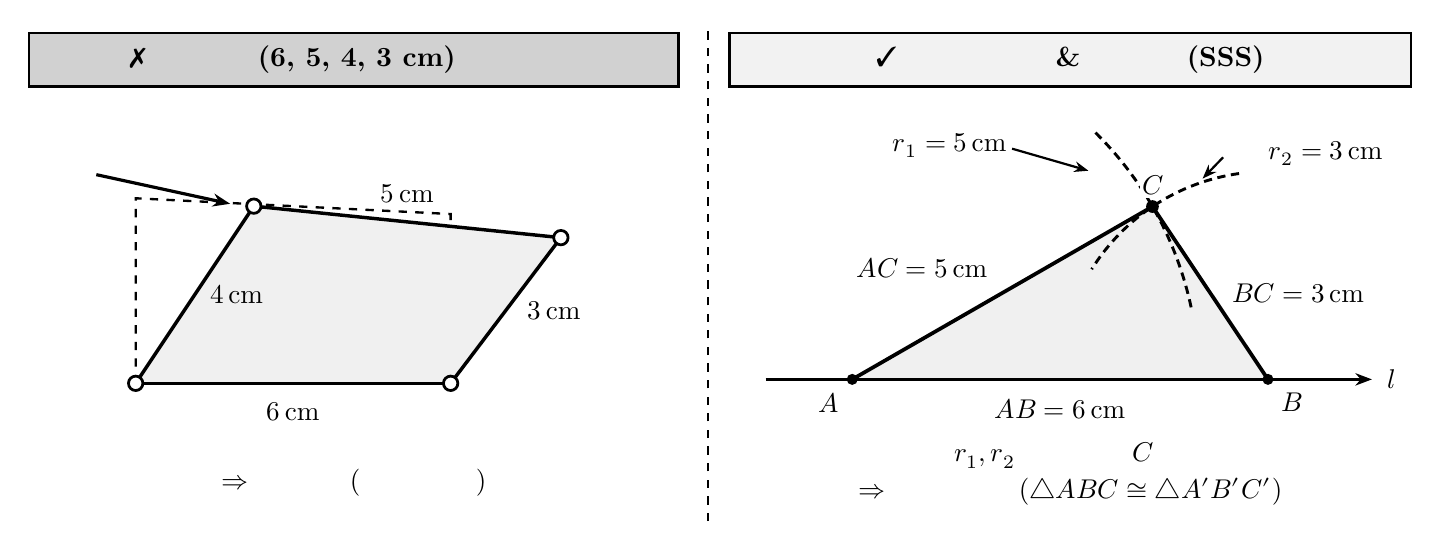
\begin{tikzpicture}[x=1cm, y=1cm, every node/.style={font=\fontsize{9.8pt}{13.5pt}\selectfont, text=black}]
  % --- ផ្នែកឆ្វេង៖ ស៊ុម ៤ របារ (6, 5, 4, 3 cm) ទ្រេតដួល (x: 0.0..8.35) ---
  \begin{scope}[shift={(0.0, 0.0)}]
    \node[draw=black, fill=midgray, line width=0.95pt, minimum width=8.25cm, minimum height=0.68cm, anchor=south, font=\fontsize{10pt}{13.8pt}\selectfont] at (4.12, 4.45) {\textbf{\ding{55}\ ស៊ុម ៤ របារ (\en{6, 5, 4, 3 cm}) ៖ មុំប្រែទ្រេត}};
    \coordinate (P1) at (1.35, 0.70);
    \coordinate (P2) at (5.35, 0.70);
    \coordinate (P3) at (6.75, 2.55);
    \coordinate (P4) at (2.85, 2.95);
    \draw[black, line width=0.85pt, dashed] (P1) -- (1.35, 3.05) -- (5.35, 2.85) -- (P2);
    \fill[panelgray] (P1) -- (P2) -- (P3) -- (P4) -- cycle;
    \draw[black, line width=1.25pt] (P1) -- (P2) node[midway, below=3pt] {$6\unit{cm}$};
    \draw[black, line width=1.25pt] (P2) -- (P3) node[midway, right=4pt] {$3\unit{cm}$};
    \draw[black, line width=1.25pt] (P3) -- (P4) node[midway, above=3pt] {$5\unit{cm}$};
    \draw[black, line width=1.25pt] (P4) -- (P1) node[midway, right=4pt, fill=panelgray, inner sep=1pt] {$4\unit{cm}$};
    \foreach \p in {P1,P2,P3,P4} {
      \fill[white, draw=black, line width=1.0pt] (\p) circle (2.6pt);
    }
    \draw[black, line width=1.15pt, -{Stealth[length=2.2mm]}] (0.85, 3.35) -- (2.55, 2.98);
    \node[anchor=south, fill=white, inner sep=1.5pt] at (1.45, 3.38) {កម្លាំងរុញ};
    \node[align=center] at (4.12, -0.45) {ស្គាល់ ៤ ជ្រុងតែគ្មានអង្កត់ទ្រូងចាក់សោ\\$\Rightarrow$ មុំប្រែសេរី (ទ្វារ ឬគ្រោងដួល)};
  \end{scope}

  % បន្ទាត់បំបែកកណ្ដាល
  \draw[black, dashed, line width=0.95pt] (8.62, -1.05) -- (8.62, 5.20);

  % --- ផ្នែកស្ដាំ៖ ស៊ុម ៣ របារ (6, 5, 3 cm) & ប្រសព្វធ្នូដែកឈាន (x: 8.90..17.65) ---
  \begin{scope}[shift={(8.90, 0.0)}]
    \node[draw=black, fill=headgray, line width=0.95pt, minimum width=8.65cm, minimum height=0.68cm, anchor=south, font=\fontsize{10pt}{13.8pt}\selectfont] at (4.32, 4.45) {\textbf{\ding{51}\ គ្រោងដំបូល ៣ របារ \en{\&} ប្រសព្វធ្នូ (\en{SSS})}};
    % មាត្រដ្ឋាន 0.88x នៃ 6, 5, 3 cm => AB = 5.28, x_C = 3.813, y_C = 2.195
    \coordinate (A) at (1.55, 0.75);
    \coordinate (B) at (6.83, 0.75);
    \coordinate (C) at (5.363, 2.945);
    \draw[black, line width=0.9pt, -{Stealth[length=2.1mm]}] (0.45, 0.75) -- (8.15, 0.75) node[right=2pt] {$l$};
    \fill[panelgray] (A) -- (B) -- (C) -- cycle;
    % ធ្នូកាំ r1=4.40 (ផ្ចិត A) និង r2=2.64 (ផ្ចិត B)
    \draw[black, line width=1.05pt, densely dashed] ($(A)+(12:4.40)$) arc (12:46:4.40);
    \draw[black, line width=1.05pt, densely dashed] ($(B)+(98:2.64)$) arc (98:148:2.64);
    \draw[black, line width=1.35pt] (A) -- (B) node[midway, below=3pt] {$AB = 6\unit{cm}$};
    \draw[black, line width=1.35pt] (A) -- (C) node[midway, above left=2pt] {$AC = 5\unit{cm}$};
    \draw[black, line width=1.35pt] (B) -- (C) node[midway, right=4pt] {$BC = 3\unit{cm}$};
    \fill[black] (A) circle (2.0pt) node[below left=2pt] {$A$};
    \fill[black] (B) circle (2.0pt) node[below right=2pt] {$B$};
    \fill[black] (C) circle (2.3pt) node[above=3pt, fill=white, inner sep=1pt] {$C$};
    \node[anchor=east, fill=white, inner sep=1pt] at (3.55, 3.72) {ធ្នូ $r_1=5\unit{cm}$};
    \draw[black, line width=0.8pt, -{Stealth[length=1.8mm]}] (3.58, 3.68) -- (4.55, 3.40);
    \node[anchor=west, fill=white, inner sep=1pt] at (6.30, 3.62) {ធ្នូ $r_2=3\unit{cm}$};
    \draw[black, line width=0.8pt, -{Stealth[length=1.8mm]}] (6.26, 3.57) -- (6.00, 3.30);
    \node[align=center] at (4.32, -0.45) {ធ្នូ $r_1, r_2$ កាត់គ្នាត្រង់ $C$ តែ \textbf{១ គត់}\\$\Rightarrow$ ចាក់សោមុំទាំង ៣ ($\tri{ABC}\cg\tri{A'B'C'}$)};
  \end{scope}
\end{tikzpicture}}

% រូបទី ២ (ផ្នែក ៥.ខ)៖ អន្ទាក់ ម.ម.ម (AAA 60°) 4cm vs 6cm និងលក្ខខណ្ឌមិនកើត 2+2.5<6
\newcommand{\figGuidelineAAAvsImpossible}{%
\linespread{1.0}\selectfont
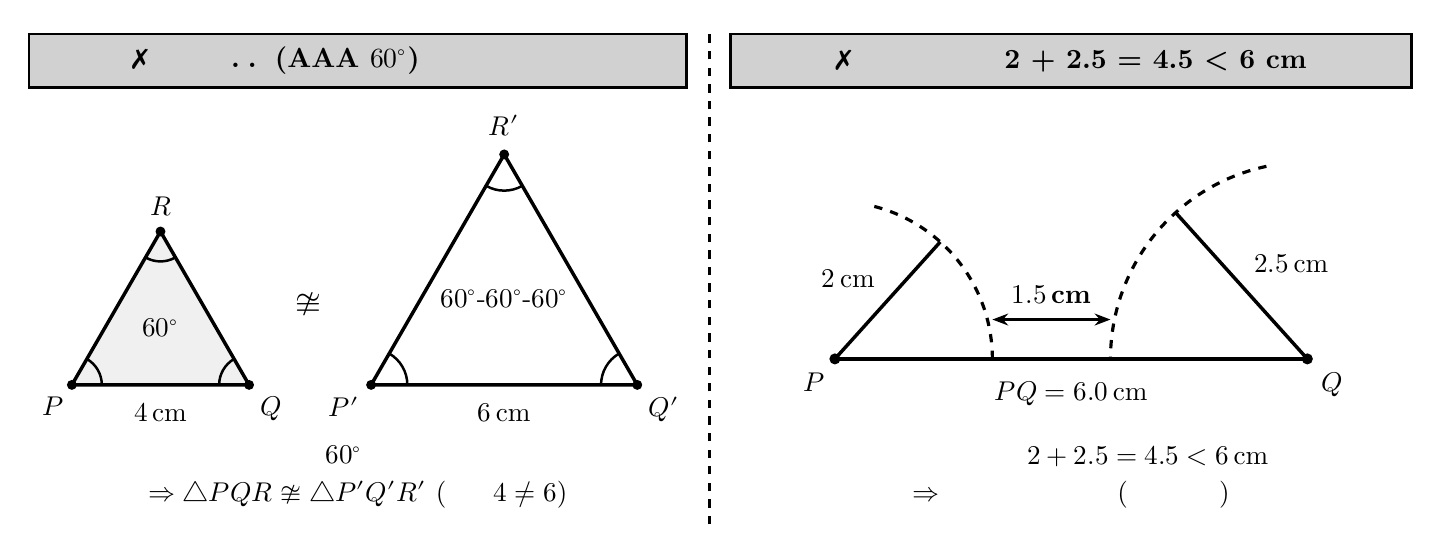
\begin{tikzpicture}[x=1cm, y=1cm, every node/.style={font=\fontsize{9.8pt}{13.5pt}\selectfont, text=black}]
  % --- ផ្នែកឆ្វេង៖ អន្ទាក់ AAA 60° (4 cm vs 6 cm) ---
  \begin{scope}[shift={(0.0, 0.0)}]
    \node[draw=black, fill=midgray, line width=0.95pt, minimum width=8.35cm, minimum height=0.68cm, anchor=south, font=\fontsize{10pt}{13.8pt}\selectfont] at (4.18, 4.48) {\textbf{\ding{55}\ អន្ទាក់ ម.ម.ម (\en{AAA} $60^\circ$) ៖ ដូចគ្នា តែមិនប៉ុន}};
    % ត្រីកោណតូច 4 cm (side 2.25)
    \coordinate (P) at (0.55, 0.72);
    \coordinate (Q) at (2.80, 0.72);
    \coordinate (R) at (1.675, 2.668);
    \fill[panelgray] (P) -- (Q) -- (R) -- cycle;
    \draw[black, line width=1.25pt] (P) -- (Q) -- (R) -- cycle;
    \pic[draw=black, line width=0.9pt, angle radius=3.8mm]{angle=Q--P--R};
    \pic[draw=black, line width=0.9pt, angle radius=3.8mm]{angle=R--Q--P};
    \pic[draw=black, line width=0.9pt, angle radius=3.8mm]{angle=P--R--Q};
    \node at (1.675, 1.44) {$60^\circ$};
    \node[below=3pt] at (1.675, 0.72) {$4\unit{cm}$};
    \fill[black] (P) circle (1.8pt) node[below left=1pt] {$P$};
    \fill[black] (Q) circle (1.8pt) node[below right=1pt] {$Q$};
    \fill[black] (R) circle (1.8pt) node[above=2pt] {$R$};

    \node[font=\fontsize{12pt}{14pt}\selectfont] at (3.55, 1.75) {$\ncg$};

    % ត្រីកោណធំ 6 cm (side 3.38, ratio 2:3)
    \coordinate (Pp) at (4.35, 0.72);
    \coordinate (Qp) at (7.73, 0.72);
    \coordinate (Rp) at (6.04, 3.647);
    \fill[white] (Pp) -- (Qp) -- (Rp) -- cycle;
    \draw[black, line width=1.25pt] (Pp) -- (Qp) -- (Rp) -- cycle;
    \pic[draw=black, line width=0.9pt, angle radius=4.6mm]{angle=Qp--Pp--Rp};
    \pic[draw=black, line width=0.9pt, angle radius=4.6mm]{angle=Rp--Qp--Pp};
    \pic[draw=black, line width=0.9pt, angle radius=4.6mm]{angle=Pp--Rp--Qp};
    \node at (6.04, 1.82) {$60^\circ\text{-}60^\circ\text{-}60^\circ$};
    \node[below=3pt] at (6.04, 0.72) {$6\unit{cm}$};
    \fill[black] (Pp) circle (1.8pt) node[below left=1pt] {$P'$};
    \fill[black] (Qp) circle (1.8pt) node[below right=1pt] {$Q'$};
    \fill[black] (Rp) circle (1.8pt) node[above=3pt] {$R'$};

    \node[align=center] at (4.18, -0.45) {មុំទាំង ៣ ស្មើ $60^\circ$ គ្រាន់តែរូប\textbf{ដូចគ្នា}\\$\Rightarrow \tri{PQR} \ncg \tri{P'Q'R'}$ (ជ្រុង $4 \neq 6$)};
  \end{scope}

  % បន្ទាត់បំបែកកណ្ដាល
  \draw[black, dashed, line width=0.95pt] (8.65, -1.05) -- (8.65, 5.24);

  % --- ផ្នែកស្ដាំ៖ បន្ទះមិនប្រសព្វ 2 + 2.5 < 6 cm ---
  \begin{scope}[shift={(8.92, 0.0)}]
    \node[draw=black, fill=midgray, line width=0.95pt, minimum width=8.65cm, minimum height=0.68cm, anchor=south, font=\fontsize{10pt}{13.8pt}\selectfont] at (4.32, 4.48) {\textbf{\ding{55}\ ប្រហោងមិនជួបគ្នា៖ \en{2 + 2.5 = 4.5 < 6 cm}}};
    \coordinate (U) at (1.32, 1.05);
    \coordinate (V) at (7.32, 1.05);
    \draw[black, line width=1.45pt] (U) -- (V) node[midway, below=4pt] {$PQ = 6.0\unit{cm}$};
    \fill[black] (U) circle (2.0pt) node[below left=2pt] {$P$};
    \fill[black] (V) circle (2.0pt) node[below right=2pt] {$Q$};

    % ធ្នូកាំ 2.0 cm (U -> x=3.32) និង 2.5 cm (V -> x=4.82) -> គម្លាត 1.5 cm
    \draw[black, line width=1.15pt, dashed] ($(U)+(0:2.0)$) arc (0:78:2.0);
    \draw[black, line width=1.25pt] (U) -- ($(U)+(48:2.0)$) node[midway, above left=1pt] {$2\unit{cm}$};
    \draw[black, line width=1.15pt, dashed] ($(V)+(102:2.5)$) arc (102:180:2.5);
    \draw[black, line width=1.25pt] (V) -- ($(V)+(132:2.5)$) node[midway, above right=1pt] {$2.5\unit{cm}$};

    % គម្លាត 1.5 cm
    \draw[black, line width=1.05pt, {Stealth[length=2.0mm]}-{Stealth[length=2.0mm]}] (3.32, 1.55) -- (4.82, 1.55);
    \node[above=2pt, align=center, fill=white, inner sep=1.5pt] at (4.07, 1.62) {\textbf{ប្រហោង}\\\textbf{$1.5\unit{cm}$}};

    \node[align=center] at (4.32, -0.45) {បូកជ្រុងខ្លីទាំងពីរ $2+2.5=4.5 < 6\unit{cm}$\\$\Rightarrow$ ធ្នូទាំងពីរមិនប្រសព្វ (គ្មានត្រីកោណ)};
  \end{scope}
\end{tikzpicture}}

% រូបទី ៣ (ផ្នែក ៥.គ)៖ កំពូលឈមជ្រុងស្មើលើរូបឆ្លុះ-បង្វិល ~135° & អន្ទាក់លំហាត់ទី៩
\newcommand{\figGuidelineVertexAndTrap}{%
\linespread{1.0}\selectfont
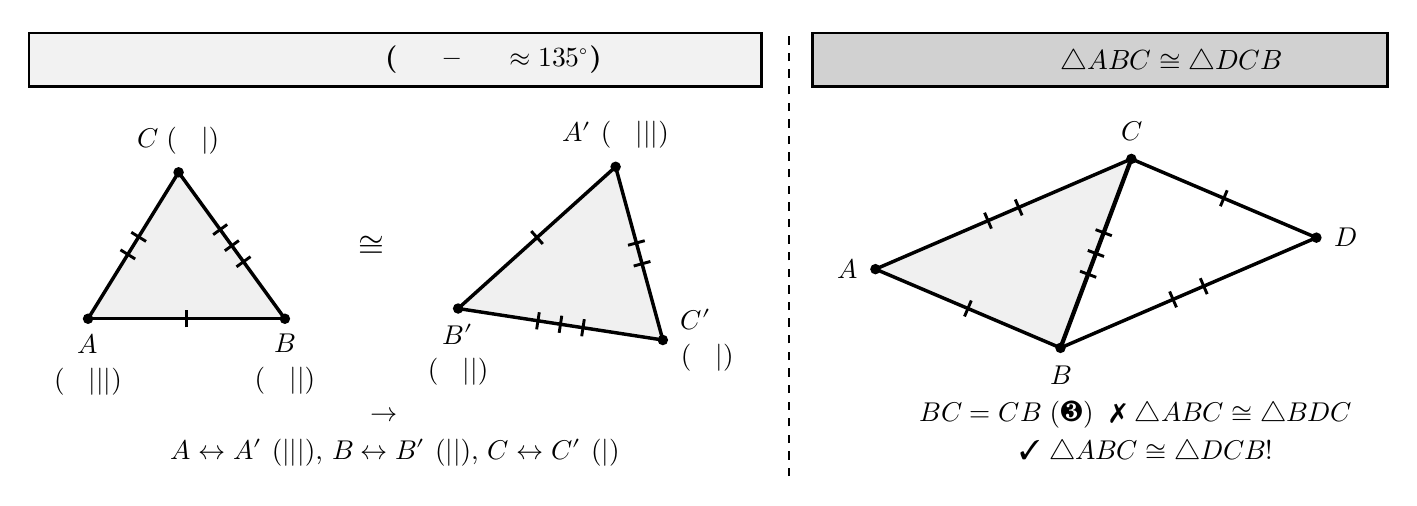
\begin{tikzpicture}[x=1cm, y=1cm, every node/.style={font=\fontsize{9.8pt}{13.5pt}\selectfont, text=black}]
  % --- ផ្នែកឆ្វេង៖ រូបបង្វិល-ឆ្លុះ ~135° & កំពូលឈមជ្រុងស្មើ (x: 0.0..9.65) ---
  \begin{scope}[shift={(0.0, 0.0)}]
    \node[draw=black, fill=headgray, line width=0.95pt, minimum width=9.30cm, minimum height=0.68cm, anchor=south, font=\fontsize{10pt}{13.8pt}\selectfont] at (4.65, 3.85) {\textbf{គោលការណ៍កំពូលឈមជ្រុងស្មើ (បង្វិល\en{--}ឆ្លុះ $\approx 135^\circ$)}};
    \coordinate (A) at (0.75, 0.92);
    \coordinate (B) at (3.25, 0.92);
    \coordinate (C) at (1.90, 2.78);
    \fill[panelgray] (A) -- (B) -- (C) -- cycle;
    \draw[black, line width=1.25pt, tk1] (A) -- (B);
    \draw[black, line width=1.25pt, tk2] (A) -- (C);
    \draw[black, line width=1.25pt, tk3] (B) -- (C);
    \fill[black] (A) circle (1.9pt) (B) circle (1.9pt) (C) circle (1.9pt);
    \node[below=2pt, align=center] at (A) {$A$\\[-1pt](ឈម $|||$)};
    \node[below=2pt, align=center] at (B) {$B$\\[-1pt](ឈម $||$)};
    \node[above=3pt] at (C) {$C$ (ឈម $|$)};

    \node[font=\fontsize{12pt}{14pt}\selectfont] at (4.35, 1.85) {$\cg$};

    % ត្រីកោណទី២ ឆ្លុះ-បង្វិល ~135 deg
    \coordinate (Ap) at (7.45, 2.85);
    \coordinate (Bp) at (5.45, 1.05);
    \coordinate (Cp) at (8.05, 0.65);
    \fill[panelgray] (Ap) -- (Bp) -- (Cp) -- cycle;
    \draw[black, line width=1.25pt, tk1] (Ap) -- (Bp);
    \draw[black, line width=1.25pt, tk2] (Ap) -- (Cp);
    \draw[black, line width=1.25pt, tk3] (Bp) -- (Cp);
    \fill[black] (Ap) circle (1.9pt) (Bp) circle (1.9pt) (Cp) circle (1.9pt);
    \node[above=3pt] at (Ap) {$A'$ (ឈម $|||$)};
    \node[below=2pt, align=center] at (Bp) {$B'$\\[-1pt](ឈម $||$)};
    \node[right=3pt, align=left] at (Cp) {$C'$\\[-1pt](ឈម $|$)};

    \node[align=center] at (4.65, -0.58) {រកគំនូសស្មើ $\to$ ស្គាល់កំពូលឈម៖\\$A\leftrightarrow A'$ ($|||$), $B\leftrightarrow B'$ ($||$), $C\leftrightarrow C'$ ($|$)};
  \end{scope}

  % បន្ទាត់បំបែកកណ្ដាល
  \draw[black, dashed, line width=0.95pt] (9.65, -1.08) -- (9.65, 4.60);

  % --- ផ្នែកស្ដាំ៖ អន្ទាក់លំហាត់ទី៩ (ទំព័រ ១៦៥ — ΔABC ≅ ΔDCB) ---
  \begin{scope}[shift={(9.95, 0.0)}]
    \node[draw=black, fill=midgray, line width=0.95pt, minimum width=7.30cm, minimum height=0.68cm, anchor=south, font=\fontsize{10pt}{13.8pt}\selectfont] at (3.65, 3.85) {\textbf{អន្ទាក់លំហាត់ទី៩៖ $\tri{ABC}\cg\tri{DCB}$}};
    \coordinate (A) at (0.80, 1.55);
    \coordinate (B) at (3.15, 0.55);
    \coordinate (C) at (4.05, 2.95);
    \coordinate (D) at (6.40, 1.95);
    \fill[panelgray] (A) -- (B) -- (C) -- cycle;
    \draw[black, line width=1.25pt, tk1] (A) -- (B);
    \draw[black, line width=1.25pt, tk1] (C) -- (D);
    \draw[black, line width=1.25pt, tk2] (A) -- (C);
    \draw[black, line width=1.25pt, tk2] (B) -- (D);
    \draw[black, line width=1.55pt, tk3] (B) -- (C);
    \fill[black] (A) circle (1.9pt) node[left=3pt] {$A$};
    \fill[black] (B) circle (1.9pt) node[below=3pt] {$B$};
    \fill[black] (C) circle (1.9pt) node[above=3pt] {$C$};
    \fill[black] (D) circle (1.9pt) node[right=3pt] {$D$};
    \node[align=center] at (3.65, -0.50) {ជ្រុងរួម $BC=CB$ (\cnum{3})៖ \ding{55}\ $\tri{ABC}\cg\tri{BDC}$\\ត្រូវសរសេរ៖ \ding{51}\ $\tri{ABC}\cg\tri{DCB}$!};
  \end{scope}
\end{tikzpicture}}

% រូបទី ៤ (ផ្នែក ៥.ឃ)៖ បច្ចេកទេស [tracing] ស្ពានតភ្ជាប់អង្កត់រួម (ទំ.១៥២ ដេក & ទំ.១៥៣ ឈរ)
\newcommand{\figGuidelineSegmentBridge}{%
\linespread{1.0}\selectfont
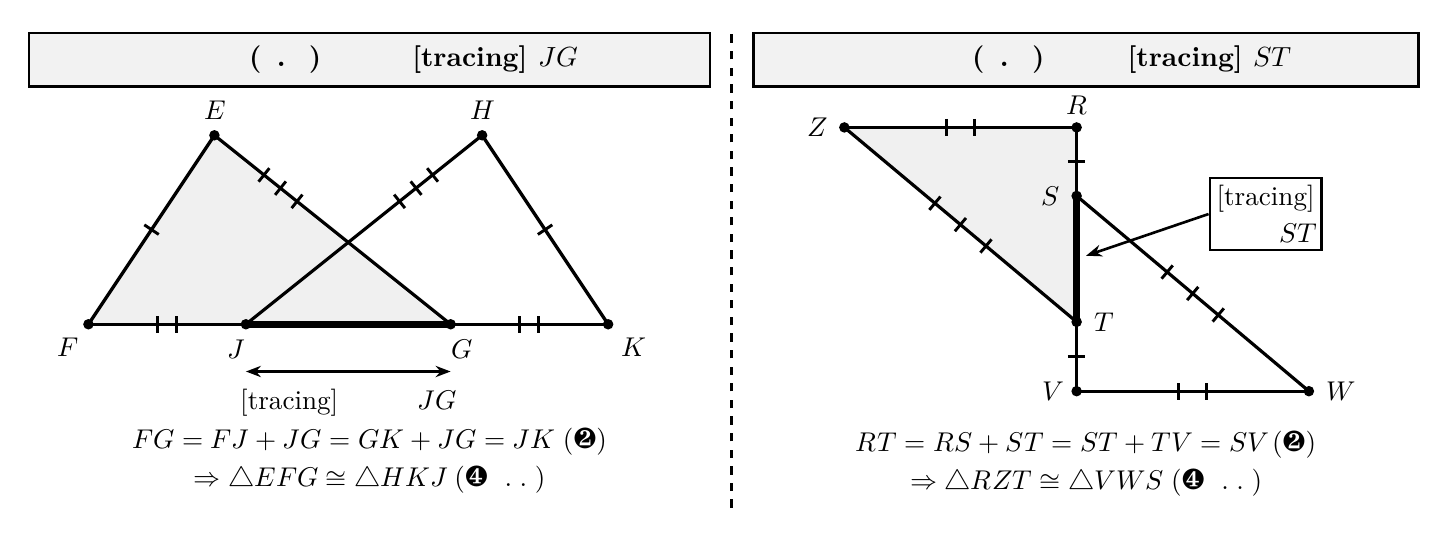
\begin{tikzpicture}[x=1cm, y=1cm, every node/.style={font=\fontsize{9.8pt}{13.5pt}\selectfont, text=black}]
  % --- ផ្នែកឆ្វេង៖ លំហាត់គំរូ (ទំ.១៥២ — F-J-G-K ដេក & ស្ពាន JG) ---
  \begin{scope}[shift={(0.0, 0.0)}]
    \node[draw=black, fill=headgray, line width=0.95pt, minimum width=8.65cm, minimum height=0.68cm, anchor=south, font=\fontsize{10pt}{13.8pt}\selectfont] at (4.32, 4.15) {\textbf{លំហាត់គំរូ (ទំ.១៥២)៖ ស្ពានដេក \en{[tracing]} $JG$}};
    \coordinate (F) at (0.75, 1.15);
    \coordinate (J) at (2.75, 1.15);
    \coordinate (G) at (5.35, 1.15);
    \coordinate (K) at (7.35, 1.15);
    \coordinate (E) at (2.35, 3.55);
    \coordinate (H) at (5.75, 3.55);
    \fill[panelgray] (E) -- (F) -- (G) -- cycle;
    \draw[black, line width=1.2pt, tk1] (E) -- (F);
    \draw[black, line width=1.2pt, tk1] (H) -- (K);
    \draw[black, line width=1.15pt, tk3u] (E) -- (G);
    \draw[black, line width=1.15pt, tk3u] (H) -- (J);
    \draw[black, line width=1.2pt, tk2] (F) -- (J);
    \draw[black, line width=1.2pt, tk2] (G) -- (K);
    \draw[black, line width=2.5pt] (J) -- (G);
    \fill[black] (F) circle (1.9pt) node[below left=2pt] {$F$};
    \fill[black] (J) circle (1.9pt) node[below=2pt, xshift=-4pt] {$J$};
    \fill[black] (G) circle (1.9pt) node[below=2pt, xshift=4pt] {$G$};
    \fill[black] (K) circle (1.9pt) node[below right=2pt] {$K$};
    \fill[black] (E) circle (1.9pt) node[above=2pt] {$E$};
    \fill[black] (H) circle (1.9pt) node[above=2pt] {$H$};
    \draw[black, line width=1.0pt, {Stealth[length=1.9mm]}-{Stealth[length=1.9mm]}] (2.75, 0.55) -- (5.35, 0.55);
    \node[below=2pt] at (4.05, 0.52) {\en{[tracing]} ស្ពានរួម $JG$};
    \node[align=center] at (4.32, -0.58) {$FG = FJ + JG = GK + JG = JK$ (\cnum{2})\\$\Rightarrow \tri{EFG}\cg\tri{HKJ}$ (\cnum{4} ជ.ជ.ជ)};
  \end{scope}

  % បន្ទាត់បំបែកកណ្ដាល
  \draw[black, dashed, line width=0.95pt] (8.92, -1.18) -- (8.92, 4.90);

  % --- ផ្នែកស្ដាំ៖ លំហាត់ប្រតិបត្តិ (ទំ.១៥៣ — R-S-T-V ឈរ & ស្ពាន ST) ---
  \begin{scope}[shift={(9.20, 0.0)}]
    \node[draw=black, fill=headgray, line width=0.95pt, minimum width=8.45cm, minimum height=0.68cm, anchor=south, font=\fontsize{10pt}{13.8pt}\selectfont] at (4.22, 4.15) {\textbf{ប្រតិបត្តិ (ទំ.១៥៣)៖ ស្ពានឈរ \en{[tracing]} $ST$}};
    \coordinate (R) at (4.10, 3.65);
    \coordinate (S) at (4.10, 2.78);
    \coordinate (T) at (4.10, 1.18);
    \coordinate (V) at (4.10, 0.30);
    \coordinate (Z) at (1.15, 3.65);
    \coordinate (W) at (7.05, 0.30);
    \fill[panelgray] (R) -- (Z) -- (T) -- cycle;
    \draw[black, line width=1.2pt, tk2] (R) -- (Z);
    \draw[black, line width=1.2pt, tk2] (V) -- (W);
    \draw[black, line width=1.15pt, tk3] (Z) -- (T);
    \draw[black, line width=1.15pt, tk3] (S) -- (W);
    \draw[black, line width=1.2pt, tk1] (R) -- (S);
    \draw[black, line width=1.2pt, tk1] (T) -- (V);
    \draw[black, line width=2.5pt] (S) -- (T);
    \fill[black] (R) circle (1.9pt) node[above=1pt] {$R$};
    \fill[black] (S) circle (1.9pt) node[left=3pt] {$S$};
    \fill[black] (T) circle (1.9pt) node[right=3pt] {$T$};
    \fill[black] (V) circle (1.9pt) node[left=3pt] {$V$};
    \fill[black] (Z) circle (1.9pt) node[left=3pt] {$Z$};
    \fill[black] (W) circle (1.9pt) node[right=3pt] {$W$};
    % ស្លាកស្ពាន ST ក្នុងចន្លោះទំនេរខាងស្ដាំលើ មិនប៉ះ SW ដាច់ខាត
    \node[draw=black, fill=white, line width=0.8pt, inner sep=2.5pt, align=center] (stlbl) at (6.50, 2.55) {\en{[tracing]}\\ស្ពានឈរ $ST$};
    \draw[black, line width=0.95pt, -{Stealth[length=2.0mm]}] (stlbl.west) -- (4.22, 2.02);
    \node[align=center] at (4.22, -0.62) {$RT = RS + ST = ST + TV = SV$ (\cnum{2})\\$\Rightarrow \tri{RZT}\cg\tri{VWS}$ (\cnum{4} ជ.ជ.ជ)};
  \end{scope}
\end{tikzpicture}}

% ============================================================================
% ចាប់ផ្ដើមឯកសារ (Document Body)
% ============================================================================
\begin{document}
\thispagestyle{firstpage}
\fontsize{11.5pt}{14.92pt}\selectfont
\vspace*{-0.75cm}

% -------------------- ក្បាលរដ្ឋបាលផ្លូវការ (Verbatim Match to LS_Plan_SSS.tex) --------------------
\begin{center}
  {\muol\fontsize{13pt}{18pt}\selectfont ព្រះរាជាណាចក្រកម្ពុជា}\\[2pt]
  {\muol\fontsize{12pt}{17pt}\selectfont ជាតិ សាសនា ព្រះមហាក្សត្រ}\\[1pt]
  \khmflourish
\end{center}

\vspace{-12pt}
{\muol\fontsize{10.8pt}{15.5pt}\selectfont
មន្ទីរអប់រំ យុវជន និងកីឡា ខេត្តកំពង់ធំ\\
ការិយាល័យអប់រំ យុវជន និងកីឡា ស្រុកកំពង់ស្វាយ\\
អនុវិទ្យាល័យព្រះក្រសាំង}

\vspace{6pt}
\begin{center}
  \parttitle{មគ្គុទ្ទេសក៍គរុកោសល្យគ្រូ និងរបាយការណ៍ស្រាវជ្រាវសង្ខេប}\\[3pt]
  {\muol\fontsize{11.5pt}{16.5pt}\selectfont ករណីត្រីកោណប៉ុនគ្នា៖ ជ្រុងបីប៉ុនរៀងគ្នា ជ\enbf{.}ជ\enbf{.}ជ \enbf{(SSS)}}
\end{center}

\vspace{4pt}

% ============================================================================
% ផ្នែកទី ១៖ ព័ត៌មានមេរៀន បរិបទកំពង់ស្វាយ និងទិដ្ឋភាពទូទៅគរុកោសល្យ
% ============================================================================
\begin{tcolorbox}[
  enhanced, sharp corners, colback=panelgray, colframe=black,
  colbacktitle=black!12, coltitle=black, titlerule=0.7pt,
  fonttitle=\fontsize{11pt}{14.5pt}\selectfont,
  fontupper=\fontsize{11.5pt}{14.92pt}\selectfont,
  title={\muol\fontsize{11pt}{14.5pt}\selectfont ព័ត៌មានទូទៅនៃមេរៀន និងកញ្ចប់ឯកសារភ្ជាប់ \enbf{(Grade 8 NGS)}},
  boxrule=1.0pt, top=6pt, bottom=6pt, left=8pt, right=8pt,
  toptitle=4pt, bottomtitle=4pt, before skip=4pt, after skip=8pt
]
  \linespread{1.0}\selectfont
  \renewcommand{\arraystretch}{1.22}
  \setlength{\tabcolsep}{1.5pt}
  \begin{tabular}{@{}L{2.80cm} L{0.20cm} L{5.25cm} L{2.50cm} L{0.20cm} L{5.40cm}@{}}
    - មុខវិជ្ជា & : & គណិតវិទ្យា ថ្នាក់ទី៨ & - រយៈពេល & : & ១ ម៉ោងសិក្សា (៥០ នាទី) \\
    - ចំណងជើងមេរៀន & : & មេរៀនទី១២ ការប្រៀបធៀបត្រីកោណ & - បង្រៀនដោយ & : & ហុក ប៊ុនថែន \\
    - ចំណងជើងរង & : & ១.២.៣ ជ្រុងបីប៉ុនរៀងគ្នា \textbf{(ជ.ជ.ជ)} & - កាលបរិច្ឆេទ & : & ថ្ងៃសុក្រ ទី២៧ ខែវិច្ឆិកា ឆ្នាំ២០២៦ \\
  \end{tabular}\\[4pt]
  \fontsize{11.5pt}{14.92pt}\selectfont\linespread{1.22}\selectfont
  \textbf{ឯកសារភ្ជាប់ក្នុងកញ្ចប់បង្រៀន (\en{NGS 5Es Lesson Package})៖}
  (១) \en{LS\_\allowbreak Plan\_\allowbreak SSS.pdf} (កិច្ចតែងការបង្រៀន ៤ ទំព័រ),
  (២) \en{Teaching\_\allowbreak Scenario\_\allowbreak SSS.pdf} (សេណារីយ៉ូ ៥០ នាទី ២ ទំព័រ),
  (៣) \en{Printable\_\allowbreak Materials\_\allowbreak SSS.pdf} (សម្ភារៈបោះពុម្ព ស-ខ្មៅ ខ្នាតពិត \en{1:1} ចំនួន ៦ ទំព័រ),
  (៤) \en{Teaching\_\allowbreak Guideline\_\allowbreak SSS.pdf} (មគ្គុទ្ទេសក៍គរុកោសល្យគ្រូនេះ),
  និង (៥) ថតភស្តុតាង ឯកសារ\allowbreak ស្រាវជ្រាវ\allowbreak យោង\_\allowbreak\en{PDF/} (\en{14 Open-Access PDFs} + \en{Evidence Index})។
\end{tcolorbox}

\secbanner{ផ្នែកទី ១៖ បរិបទមេរៀន និងទិដ្ឋភាពទូទៅគរុកោសល្យ}{Section 1: Administrative Context, Grade 8 Kampong Svay Setting \& 50-Min Overview}

\subsec{១\enbf{.}១ បរិបទថ្នាក់ទី៨ អនុវិទ្យាល័យព្រះក្រសាំង និងតម្រូវការផ្លាស់ប្ដូរវិធីសាស្រ្តបង្រៀន}

នៅអនុវិទ្យាល័យព្រះក្រសាំង (ស្រុកកំពង់ស្វាយ ខេត្តកំពង់ធំ) សិស្សថ្នាក់ទី៨ ទើបតែឆ្លងកាត់មេរៀនករណីត្រីកោណប៉ុនគ្នាពីរគឺ ម.ជ.ម (\en{ASA}) និង ជ.ម.ជ (\en{SAS}) មុនឈានដល់ \textbf{§១.២.៣ ករណី ជ្រុងបីប៉ុនរៀងគ្នា (ជ.ជ.ជ / \en{SSS})} ក្នុងសៀវភៅសិក្សាគោលថ្នាក់ទី៨ ទំព័រ \textbf{១៥១--១៥៣} (និងលំហាត់ទី៤, ទី៩ ទំព័រ \textbf{១៦៤--១៦៥})។ តាមទម្លាប់បង្រៀនប្រពៃណី គ្រូភាគច្រើនចាប់ផ្ដើមដោយសូត្រនិយមន័យ «ជ្រុង ៣ ប៉ុនគ្នា $\Rightarrow$ ត្រីកោណប៉ុនគ្នា» ភ្លាមៗ រួចចម្លងតារាងពីទំព័រ ១៥២ ដាក់លើក្ដារខៀន។ វិធីសាស្ត្រអកម្មនេះបង្កបញ្ហាធ្ងន់ធ្ងរ ៥ យ៉ាង៖
\begin{itemize}[leftmargin=0.55cm, topsep=1pt, itemsep=1.5pt, parsep=0pt]
  \item \textbf{១) មិនយល់ភាពខុសគ្នារវាង «ស៊ុម ៣ របាររឹង» និង «ស៊ុម ៤ របារទ្រេត»៖} សិស្សទន្ទេញ ជ.ជ.ជ ដោយមិនដឹងហេតុអ្វីជ្រុង ៣ ចាក់សោមុំដោយស្វ័យប្រវត្តិ (ខណៈចតុកោណស្គាល់ ៤ ជ្រុងនៅតែរង្គើដួល) និងមិនយល់ហេតុអ្វីធ្នូដែកឈាន $r_1=5\unit{cm}$ ពី $A$ និង $r_2=3\unit{cm}$ ពី $B$ កំណត់ចំណុច $C$ តែមួយគត់លើម្ខាងអ័ក្ស $l$ \en{(Zhang, 2017; Demiray et al., 2023)}។
  \item \textbf{២) អន្ទាក់ ម.ម.ម (\en{AAA}) និងលក្ខខណ្ឌមិនបង្កើតត្រីកោណ ($2+2.5<6$)៖} សិស្សស្មានថា «បើជ្រុង ៣ ប៉ុនគ្នាធានាប៉ុនគ្នា នោះមុំ ៣ ប៉ុនគ្នាក៏ប្រាកដជាប៉ុនគ្នាដែរ» ដោយច្រឡំភាពដូចគ្នា (\en{Similarity}) ជាមួយភាពប៉ុនគ្នា (\en{Congruence}) \en{(Dündar \& Gündüz, 2017; Shahbari \& Daher, 2020)}។
  \item \textbf{៣) ការធ្លាក់ចុះធ្ងន់ធ្ងរលើរូបត្រួតគ្នា និងការរំលងស្ពានអង្កត់រួម៖} លើលំហាត់គំរូទំព័រ ១៥២ ($F\text{-}J\text{-}G\text{-}K$) និងប្រតិបត្តិទំព័រ ១៥៣ ($R\text{-}S\text{-}T\text{-}V$) សិស្សតែងភ្លេចបូកអង្កត់រួម $JG$ ឬ $ST$ ហើយអត្រាត្រឹមត្រូវលើ \en{S.S.S.} ធ្លាក់ពី $84\%$ មកត្រឹម $49\%$ ពេលត្រីកោណត្រួតគ្នា \en{(Biber, 2020)}។
  \item \textbf{៤) កំហុសលំដាប់កំពូលលើរូបឆ្លុះ-បង្វិល និងកំហុសបោះពុម្ពសៀវភៅគោល៖} ពេលត្រីកោណឆ្លុះ-បង្វិល $\approx 135^\circ$ សិស្សច្រឡំលំដាប់អក្សរកំពូល \en{(Ubah \& Bansilal, 2019)} ជាពិសេសក្នុង\textbf{លំហាត់ទី៩ ទំព័រ ១៦៥} ដែលប្រធានសរសេរ «ប្រៀបធៀប $\tri{ABC}$ និង $\tri{BDC}$» ទាំងដែលកំពូលពិតគឺ $\tri{ABC} \cg \tri{DCB}$។ បន្ថែមពីនេះ \textbf{តារាងទំព័រ ១៥២} បោះពុម្ពភ័ន្តជា $AB = B'C'$ (ជួរទី ៣) ជំនួសឱ្យ \textbf{$BC = B'C'$} និងក្នុងកថាខណ្ឌសរសេរថា «ម្ខាងនៃជ្រុង $A'C'$» ជំនួសឱ្យ \textbf{$A'B'$}។
  \item \textbf{៥) ដែនកំណត់ក្រដាសថតចម្លង ស-ខ្មៅ នៅតាមសាលារៀនជនបទ៖} ឯកសារព្រីនក្នុងសាលារៀនជាទូទៅជា ស-ខ្មៅ (គ្មានពណ៌)។ ដូច្នេះមេរៀននេះជំនួសហ្វឺតពណ៌ទាំងស្រុងដោយ\textbf{គំនូស ស-ខ្មៅ ($|, \parallel, |||$) + ការចង្អុលម្រាមដៃ \en{[tracing]} + ធនាគារហេតុផល \cnum{1}--\cnum{5}} \en{(Yeo \& Tzeng, 2019)}។
\end{itemize}

\subsec{១\enbf{.}២ ដំណើរសាច់រឿង ៥០ នាទី \enbf{(2 + 9 + 17 + 20 + 2 min)} និងសមាហរណកម្មកញ្ចប់ឯកសារ ៤}

មេរៀនត្រូវបានរៀបចំតាមរយៈពេលស្តង់ដារ \textbf{៥០ នាទីពេញ} ក្រោមបរិបទជាក់ស្ដែងនៅស្រុកកំពង់ស្វាយ («\textbf{ក្រុមជាងសំណង់ដំបូល}» ៣ នាក់/ក្រុម) ដោយសមកាលកម្ម ១០០\% រវាង \en{LS\_\allowbreak Plan\_\allowbreak SSS.tex}, \en{Teaching\_\allowbreak Scenario\_\allowbreak SSS.tex}, និង \en{Printable\_\allowbreak Materials\_\allowbreak SSS.pdf} (ទំព័រ ១--៦)៖
\begin{itemize}[leftmargin=0.55cm, topsep=1pt, itemsep=1.5pt, parsep=0pt]
  \item \textbf{ជំហានទី ១ (00--02 min | ២ នាទី)៖} រដ្ឋបាលថ្នាក់ និងចាត់ក្រុម «ក្រុមជាងសំណង់ដំបូល» ៣ នាក់ ចែកកញ្ចប់សម្ភារៈកាត់ខ្នាត \en{1:1} (ទំព័រ ១) បិទជិតលើតុ។
  \item \textbf{ជំហានទី ២ (02--11 min | ៩ នាទី = ៣ + ៣ + ៣)៖} (ក) កំណែកិច្ចការផ្ទះ ម.ជ.ម ដោយ\textbf{ល្បែងចាប់កំហុស} ($\tri{ABC}$ សមបាទ, សំណួរបញ្ឆោត $AB=AC$ ក្នុង $\tri{BDE}, \tri{CDE}$); (ខ) រំលឹករហ័ស ២ ភាគ (ធ្នូកាំ $5\unit{cm}$ ផ្ចិត $A$ និងបូកអង្កត់ត្រង់ជួរ $F\text{-}J\text{-}G\text{-}K$); (គ) \textbf{\en{E1 Engage}}៖ រឿងជាងឈើកំពង់ស្វាយធ្វើគ្រោងដំបូល $6\unit{m}, 5\unit{m}, 3\unit{m}$ ដូចគ្នាដោយ\textbf{គ្មានរ៉ាព័រទ័រ} ធៀបនឹងទ្វារ ៤ របារទ្រេតដួល។
  \item \textbf{ជំហានទី ៣ (11--28 min | ១៧ នាទី = ១១ + ៦)៖} \textbf{\en{E2 Explore (11 min)}}៖ សកម្មភាព ១ (តេស្តស៊ុម ៤ របារ $6,5,4,3\unit{cm}$ vs ៣ របារ $6,5,3\unit{cm}$ + គូសធ្នូដែកឈាន $r_1=5, r_2=3\unit{cm}$ ប្រសព្វត្រង់ $C$ តែ ១ + ត្រួតបង្វិល-ត្រឡប់ក្រដាសកាត់) និងសកម្មភាព ២ (\en{POE} អន្ទាក់ ម.ម.ម \en{AAA} $60^\circ$ $4\unit{cm}$ vs $6\unit{cm}$ + បន្ទះ $2, 2.5, 6\unit{cm}$); \textbf{\en{E3 Explain (6 min)}}៖ បង្គុំទ្រឹស្ដីបទ ជ.ជ.ជ លើរូបបង្វិល-ឆ្លុះ $\approx 135^\circ$, \textbf{គោលការណ៍កំពូលឈមជ្រុងស្មើ}, កែតារាងទំព័រ ១៥២ ($AB=B'C' \to BC=B'C'$), ធនាគារហេតុផល \cnum{1}--\cnum{5} (ទំព័រ ៤) និងញែក $=$ ទល់ $\cg$។
  \item \textbf{ជំហានទី ៤ (28--48 min | ២០ នាទី = ១០ + ១០)៖} \textbf{\en{E4 Elaborate (10 min)}}៖ លំហាត់គំរូទំព័រ ១៥២ ($F\text{-}J\text{-}G\text{-}K$) ដោយប្រើកាត «ស្ពានតភ្ជាប់អង្កត់ $JG$ និងគំនូស $|, \parallel, |||$» (ទំព័រ ២) ម្រាមដៃ \en{[tracing]} + ៣០ វិនាទី \en{EIA Looking-Back}; \textbf{\en{E5 Evaluate (10 min)}}៖ ប្រលង «ក្រុមអធិការកិច្ចប្លង់ ៣ តួនាទី» (៧ នាទី, ទំព័រ ៣) លើប្រតិបត្តិទំព័រ ១៥៣ ($R\text{-}S\text{-}T\text{-}V$) ភ្ជាប់ \en{Pause-Ask / Pause-Review} និងបិទបេសកកម្មដំបូល \en{E1}, បន្តដោយ «កាតត្រួតពិនិត្យ \en{A--D}» (៣ នាទី / 60--90s, ទំព័រ ៥)។
  \item \textbf{ជំហានទី ៥ (48--50 min | ២ នាទី)៖} ចែកប័ណ្ណកិច្ចការផ្ទះ ៤-up (ទំព័រ ៦)៖ លំហាត់ទី៤ (ទំ.១៦៤ ខ្លែង $ABCD$) និងលំហាត់ទី៩ (ទំ.១៦៥ ចតុកោណ $ABDC$, ផ្ទៀង $\tri{ABC}\cg\tri{DCB}$) ព្រមទាំងបណ្ដាំផ្ញើសុវត្ថិភាព។
\end{itemize}

% ============================================================================
% ផ្នែកទី ២៖ ការសំយោគឯកសារស្រាវជ្រាវអន្តរជាតិ (14 Verified OA PDFs)
% ============================================================================
\secbanner{ផ្នែកទី ២៖ ការសំយោគឯកសារស្រាវជ្រាវអន្តរជាតិ \enbf{(Mini-Literature Review)}}{Section 2: Research-to-Practice Rationale Grounded in 14 Verified Open-Access PDFs}

រាល់សកម្មភាព សំណួរផ្អាក សម្ភារៈកាត់ និងបច្ចេកទេសបង្ការកំហុសក្នុងមេរៀន \en{SSS} ៥០ នាទីនេះ ត្រូវបានសំយោគផ្ទាល់ពីអត្ថបទស្រាវជ្រាវអន្តរជាតិ \en{Open-Access} ចំនួន \textbf{១៤ អត្ថបទ} (ផ្ទៀងផ្ទាត់អត្ថបទពេញតាម \en{PyMuPDF} ក្នុងថត ឯកសារស្រាវជ្រាវយោង\_\en{PDF/}) ដូចខាងក្រោម៖

\subsec{២\enbf{.}១ ភាពរឹងមាំគ្រោងត្រីកោណ \enbf{CRA} បទពិសោធន៍ផ្ទាល់ដៃ និងការសង់ដោយដែកឈាន}

\begin{itemize}[leftmargin=0.50cm, topsep=2pt, itemsep=2.5pt, parsep=0pt]
  \item \textbf{លំដាប់ \en{Concrete--Representational--Abstract (CRA)} ចំគោលដៅ \en{SSS}៖} ក្នុងការសិក្សាពហុមូលដ្ឋាន (\en{N=4} សិស្សមានបញ្ហាធរណីមាត្រ) \en{Zhang (2017)} បញ្ជាក់ថាការហ្វឹកហាត់ចងចាំរូបភាព (\en{Phase 1 VWM}) តែឯងមិនធ្វើឱ្យសិស្សចេះបែងចែកឬដោះស្រាយបញ្ហាត្រីកោណប៉ុនគ្នាទេ។ លុះត្រាតែបន្ថែមការបង្រៀនតាមលំដាប់ \en{CRA} ក្នុង \en{Phase 2} — ដោយឱ្យសិស្សផ្គុំ\textbf{ដំបងប្រវែងថេរ (`3, 4, 5` ឯកតា)} សាកល្បងបង្កើតត្រីកោណទី២ ខុសគ្នា (តែមិនអាចទៅរួច) មុនបង្វិលត្រួតរូប (\en{Representational}) និងសូត្រទ្រឹស្ដីបទ (\en{Abstract}) — ទើបភាពត្រឹមត្រូវកំណត់អត្តសញ្ញាណប៉ុនគ្នាហក់ឡើងពី $75\%\to 100\%$ (\en{Tanya}), $33\%\to 93\%$ (\en{Monica}), $33\%\to 67\%$ (\en{Nicky}) និងការដោះស្រាយបញ្ហាកើនពី $42\%\to 83\%$, $47\%\to 83\%$, $33\%\to 100\%$, និង $53\%\to 67\%$។ លទ្ធផលនេះគាំទ្រដោយផ្ទាល់នូវពិសោធន៍ ១ ក្នុង \en{E2} ដែលឱ្យសិស្សតភ្ជាប់របារ $6, 5, 3\unit{cm}$ ធៀបនឹង ៤ របារ $6, 5, 4, 3\unit{cm}$។
  \item \textbf{ភស្តុតាងសរសៃប្រសាទ \en{fNIRS} និងបរិបទរចនាដំបូល \en{RME}៖} \en{Shi et al. (2023)} (\en{n=38}, អាយុមធ្យម $13.58$ ឆ្នាំ) វាស់ដោយឧបករណ៍ \en{fNIRS} បង្ហាញថាការកាន់បត់បង្វិលសម្ភារៈផ្ទាល់ដៃឈ្នះការមើលវីដេអូអកម្មយ៉ាងមានន័យ ($F(1, 34) = 22.31, p < .001, \eta^2_p = .39$) ជាពិសេសសម្រាប់សិស្សរៀនយឺត (\en{Operation+L}: $M = 4.80, SD = 1.23$ ទល់នឹង $2.56$) ដោយជំរុញតំបន់វិញ្ញាណ-ចលនា (\en{SAC}, $\eta^2_p = .23$; \en{left PMC}, $\eta^2_p = .29$) និងបន្ថយបន្ទុកគិតលើ \en{left DLPFC} ($\eta^2_p = .23$)។ ចំណែក \en{Fahrurozi et al. (2018)} តាមគន្លង \en{RME / PMRI} ចាប់ផ្ដើមពីរចនាសម្ព័ន្ធដំបូលស្ថាបត្យកម្មក្នុងសហគមន៍ (\en{Horizontal}) ឆ្លងទៅការបំប្លែងរឹងផ្ទៀងភាពប៉ុនគ្នា (\en{Vertical}) — ដែលជំរុញឱ្យយើងយក\textbf{គ្រោងដំបូលផ្ទះកំពង់ស្វាយ ($6, 5, 3\unit{m}$)} មកបើកឆាក \en{E1} និងបិទបេសកកម្មនៅ \en{E5}។
  \item \textbf{អំណះអំណាងពេលសង់ដោយដែកឈាន និងបន្ទាត់ត្រង់៖} \en{Demiray et al. (2023)} វិភាគការពិភាក្សាជាក្រុម ($N=14$, ៤ ក្រុម) លើសកម្មភាពសង់ធរណីមាត្រ ហើយបន្ថែមធាតុ ៥ ទៀតលើគំរូ \en{Toulmin} (\en{conclusion/data, target conclusion, guidance, challenger, objection})។ ការសិក្សានេះបង្ហាញថាក្រុមប្រើដែកឈាន និងបន្ទាត់ត្រង់ងាយជាប់គាំងនៅពេលត្រូវពន្យល់មូលហេតុធ្នូប្រសព្វ បើខ្វះ \en{Guidance} ពីគ្រូអំពីគន្លងចំណុចស្មើចម្ងាយ (\en{Equidistant Locus})។ ហេតុនេះ មេរៀនយើងភ្ជាប់\textbf{រំលឹកទី១} (ធ្នូកាំ $5\unit{cm}$ ផ្ចិត $A$) ជាមួយ\textbf{សំណួរដឹកនាំ}ពេលប្រសព្វធ្នូ $r_1=5\unit{cm}, r_2=3\unit{cm}$ ត្រង់ $C$ ក្នុង \en{E2}។
\end{itemize}

\subsec{២\enbf{.}២ ការញែកអន្ទាក់ \enbf{AAA} ចេញពី \enbf{SSS} និងវិបត្តិលំដាប់កំពូលលើរូបឆ្លុះ\enbf{-}បង្វិល}

\begin{itemize}[leftmargin=0.50cm, topsep=2pt, itemsep=2.5pt, parsep=0pt]
  \item \textbf{អន្ទាក់ ម.ម.ម (\en{AAA}) និងកង្វះការផ្ដល់ហេតុផលផ្លូវការ៖} \en{Dündar \& Gündüz (2017)} វាយតម្លៃអ្នកចូលរួម $N=46$ លើសំណួរ \en{SSS} ធៀបនឹង \en{AAA Similarity} (\en{GCKQ, GJP, GQDLE}) ហើយរកឃើញថាអត្រាទាំងឆ្លើយត្រូវនិងផ្ដល់ហេតុផលពេញលេញគឺ\textbf{ក្រោម $50\%$} គ្រប់សំណួរទាំងអស់ (ខ្ពស់បំផុតលើ \en{Q1 SSS} មាន $23/46$, ដោយច្រើនពឹងលើការពិសោធន៍ជាក់ស្ដែងជាងពាក្យគន្លឹះផ្លូវការ, រីឯ \en{Q4} មាន $12.1\%$ ឆ្លើយត្រូវតែហេតុផលខុស)។ ទន្ទឹមគ្នានេះ \en{Shahbari \& Daher (2020)} សិក្សាលើសិស្សរៀនយឺត $N=30$ បង្ហាញថាការកាត់និងត្រួតផ្ទៀងត្រីកោណដោយដៃផ្ទាល់លើកពិន្ទុពី $M=15.9$ ($SD=10.137$) ដល់ $M=88.6$ ($SD=11.57$), $t(29)=-17.14, p<.001$ ហើយឱ្យសិស្សច្រានចោលលក្ខខណ្ឌ \en{equality in three angles (AAA)} ដោយខ្លួនឯង។ ដូច្នេះ \en{E2 Act 2} ប្រើ \en{POE} កាត់ត្រួតត្រីកោណសម័ង្ស $60^\circ$ ($4\unit{cm}$ ទល់ $6\unit{cm}$) ដើម្បីបំបាក់អន្ទាក់ ម.ម.ម ភ្លាមៗ។
  \item \textbf{កម្រិតគិត \en{Van Hiele} ទាប និងការធ្លាក់ចុះ $21.5\%$ លើរូបឆ្លុះ-បង្វិល៖} \en{Manalo (2025)} វាយតម្លៃសិស្សថ្នាក់ទី៨ $N=109$ រកឃើញថា $74.32\%$ នៅកម្រិតទាប (\en{Task 1}: $38.54\%$ \en{L0} + $35.78\%$ \en{L1}; មានតែ $5.50\%$ \en{L3} និង $0\%$ \en{L4}) និង $85.32\%$ ជាប់នៅ \en{L0} លើ \en{Task 3}។ ពាក់ព័ន្ធផ្ទាល់នឹងទិសដៅរូប \en{Ubah \& Bansilal (2019)} ($N=65$, ទ្រឹស្ដី \en{Duval Semiotic Registers}) រកឃើញថាពេលត្រីកោណមានទិសដៅឆ្លុះ (\en{Q2.7 reflected}) អត្រាឆ្លើយត្រូវធ្លាក់ចុះមកត្រឹម \textbf{$21.5\%$ ($14/65$)} និងខុសដល់ \textbf{$64.6\%$ ($42/65$)} ធៀបនឹងទិសដៅត្រង់ \en{Q2.2} ($60.0\%$, $39/65$) ដោយសិស្សសរសេរលំដាប់កំពូលខុស ($\tri{ABE}$ vs $\tri{DCE}$) រហូតដល់បានប្រើក្រដាសកាត់បង្វិលផ្គូផ្គងមុំ/ជ្រុងឈម។ ភស្តុតាងនេះឆ្លើយតប ១០០\% ទៅនឹងការបង្វិល-ឆ្លុះ $\approx 135^\circ$ ក្នុង \en{E3} និងការជួយសិស្សដោះ\textbf{អន្ទាក់លំហាត់ទី៩} ($\tri{ABC}\cg\tri{DCB}$ ជំនួស $BDC$)។
\end{itemize}

\subsec{២\enbf{.}៣ អន្ទាក់ \enbf{SSS} ត្រួតគ្នា ទម្រង់ \enbf{Flow-Chart + 3} បន្ទាត់ និងម្រាមដៃ \enbf{[tracing]}}

\begin{itemize}[leftmargin=0.50cm, topsep=2pt, itemsep=2.5pt, parsep=0pt]
  \item \textbf{ការធ្លាក់ចុះពី $84\%$ មក $49\%$ លើលំហាត់ \en{SSS} ត្រួតលើគ្នា៖} \en{Biber (2020)} ($N=55$) បញ្ជាក់ក្នុង \en{Table 2} ថាភាពត្រឹមត្រូវលើករណី \textbf{\en{S.S.S.}} មាន $84\%$ ($46/55$) លើរូបដាច់ដោយឡែក និង $80\%$ ($44/55$) លើរូបជាប់គ្នា ប៉ុន្តែ\textbf{ធ្លាក់ចុះដល់ $49\%$ ($27/55$)} នៅពេលត្រីកោណត្រួតលើគ្នា ($4/5$ សិស្សសម្ភាសន៍ខុសលំហាត់ទី ៩) — ដូចរូបទំព័រ ១៥២ ($F\text{-}J\text{-}G\text{-}K$) និងទំព័រ ១៥៣ ($R\text{-}S\text{-}T\text{-}V$) នៃសៀវភៅគោលខ្មែរ។
  \item \textbf{ចន្លោះប្រហោង \en{FG1} និងការច្រឡំ $=$ vs $\cg$៖} \en{Winer \& Battista (2022)} វិភាគភស្តុតាង $84$ សន្លឹក រកឃើញថាមានតែ $18\%$ ($15/84$) គ្មានចន្លោះប្រហោង; $49\%$ ($81/165$) ជាកំហុស \en{FG1} (គ្រាន់តែគូសលើរូបហើយលោតរំលងអនុអំណះអំណាង); និង $64\%$ ($52/81$) នៃ \en{FG1} ច្រឡំ $=$ (រង្វាស់/ប្រវែង) នឹង $\cg$ (ត្រីកោណប៉ុនគ្នា)។
  \item \textbf{ទម្រង់ \en{Flow-Chart} រួមជាមួយសំណេរ ៣ បន្ទាត់ + \en{EIA} + \en{[tracing]} ស-ខ្មៅ៖} \en{Miyazaki et al. (2014)} បង្ហាញលើសិស្សថ្នាក់ទី៨ (៩ ម៉ោង) ថាការប្រើដ្យាក្រាមលំហូរលើលំហាត់ \textbf{\en{SSS}} ($\tri{ABO}\cg\tri{ACO}$ តាម $AO=AO, AB=AC, BO=CO$) បណ្ដុះការគិតទៅមុខ-ត្រឡប់ក្រោយ និងជំរុញពិន្ទុខ្ពស់ជាងមធ្យមភាគជាតិ $+10\%$, ខណៈ \en{Miyazaki et al. (2019)} បង្កើតលំដាប់រៀបផែនការ \en{P1--P2}, ការសង់ \en{C1--C2}, និង \en{EIA Looking-Back}។ ស្របគ្នានេះ \en{Anwar et al. (2021)} ($N=125$: ក្រុមចម្រុះ $n=60$ ប្រើ \en{flow-chart} ភ្ជាប់ \en{two-column/paragraph} vs ក្រុមគ្រប់គ្រង $n=65$ ប្រើ \en{two-column} តែឯង) បង្ហាញថា \en{N-Gain} ក្រុមចម្រុះខ្ពស់ដល់ $0.733$ ($M=13.75, SD=1.781$) ធៀបនឹង $0.330$ ($M=10.80, SD=2.425$), \en{Mann-Whitney} $U(60,65)=547.5, p<.001$, ដោយ $61.7\%$ ធៀបនឹង $9.3\%$ ឈានផុតកម្រិត \en{Recognizing Elements} (និង $56.7\%$ vs $6.2\%$ ឈានដល់ \en{Beyond Chaining Elements})។ ជាចុងក្រោយ \en{Yeo \& Tzeng (2019)} ($N=72$, អាយុ $12.35$ ឆ្នាំ) បញ្ជាក់ថា\textbf{ការចង្អុលម្រាមដៃ \en{[tracing]}} លើឧទាហរណ៍គំរូបង្កើនភាពត្រឹមត្រូវបម្លែង ($M=3.00, SD=0.85$ vs $M=2.31, SD=1.01$; $F(1,68)=9.38, p=.003, \eta^2=.121$) និងកាត់បន្ថយបន្ទុកគិតស្មើភាពគ្នាគ្រប់កម្រិតចងចាំ ($p \ge .309$) — ជំនួសហ្វឺតពណ៌បាន ១០០\% លើក្រដាស ស-ខ្មៅ!
\end{itemize}

\subsec{២\enbf{.}៤ តារាងផ្ទៀងផ្គងឯកសារភស្តុតាង \enbf{PDF} ទាំង ១៤ \enbf{(Evidence Alignment Summary)}}

\begingroup
\linespread{1.0}\selectfont
\renewcommand{\arraystretch}{1.12}
\setlength{\tabcolsep}{3.0pt}
\fontsize{10.0pt}{14.0pt}\selectfont
\begin{longtable}{|C{0.65cm}|L{4.05cm}|L{2.55cm}|L{5.35cm}|L{3.90cm}|}
\hline
\rowcolor{headgray}
\multicolumn{1}{|C{0.65cm}|}{\tblhead{\enbf{\#}}} &
\multicolumn{1}{C{4.05cm}|}{\tblhead{ឯកសារ \enbf{PDF}\newline \enbf{(}ថតភស្តុតាង\enbf{)}}} &
\multicolumn{1}{C{2.55cm}|}{\tblhead{ប្រភព \enbf{APA}}} &
\multicolumn{1}{C{5.35cm}|}{\tblhead{ភស្តុតាងជាក់ស្ដែង\newline \enbf{(Verified Stats)}}} &
\multicolumn{1}{C{3.90cm}|}{\tblhead{ចំណុចអនុវត្ត\newline ក្នុងមេរៀន \enbf{SSS}}} \\
\hline
\endfirsthead

\hline
\rowcolor{headgray}
\multicolumn{1}{|C{0.65cm}|}{\tblhead{\enbf{\#}}} &
\multicolumn{1}{C{4.05cm}|}{\tblhead{ឯកសារ \enbf{PDF}\newline \enbf{(}ថតភស្តុតាង\enbf{)}}} &
\multicolumn{1}{C{2.55cm}|}{\tblhead{ប្រភព \enbf{APA}}} &
\multicolumn{1}{C{5.35cm}|}{\tblhead{ភស្តុតាងជាក់ស្ដែង\newline \enbf{(Verified Stats)}}} &
\multicolumn{1}{C{3.90cm}|}{\tblhead{ចំណុចអនុវត្ត\newline ក្នុងមេរៀន \enbf{SSS}}} \\
\hline
\endhead

\hline
\endfoot

\hline
\endlastfoot

01 & \en{01\_\allowbreak Zhang2017\_\allowbreak CRA\allowbreak TriangleSSS.pdf} & \en{Zhang (2017)} &
$N=4$ \en{GD}៖ \en{Phase 1 VWM} មិនកែ \en{Congruence}; \en{Phase 2 CRA} ដំបង $3,4,5$ កើន \en{ID} $75\to100\%$, $33\to93\%$ \& \en{PS} $42\text{--}53\% \to 67\text{--}100\%$។ &
\textbf{E2 Act 1}: តភ្ជាប់របារ $6,5,3\unit{cm}$ ទល់ ៤ របារ ($6,5,4,3\unit{cm}$), ទំព័រ ១។ \\ \hline

02 & \en{02\_\allowbreak Demiray2023\_\allowbreak Compass\allowbreak ConstructionArg.pdf} & \en{Demiray et al. (2023)} &
$N=14$ (៤ ក្រុម)៖ បន្ថែម ៥ ធាតុលើ \en{Toulmin}; ក្រុមដែកឈានត្រូវការ \en{Guidance} លើចម្ងាយស្មើ (\en{Locus})។ &
\textbf{ជំ.២ ខ \& E2}: ធ្នូកាំ $5\unit{cm}$, ប្រសព្វ $r_1=5, r_2=3\unit{cm}$ ត្រង់ $C$។ \\ \hline

03 & \en{03\_\allowbreak Miyazaki2014\_\allowbreak OpenFlow\allowbreak ChartSSS.pdf} & \en{Miyazaki et al. (2014)} &
ថ្នាក់ទី៨ (៩ ម៉ោង)៖ \en{Flow-chart} លើ \en{SSS} ($\tri{ABO}\cg\tri{ACO}$) គិតទៅមុខ-ត្រឡប់ក្រោយ ឈ្នះជាតិ $+10\%$។ &
\textbf{E3 \& E4}: រចនាកាតស្ពាន \cnum{1}--\cnum{5} ទំព័រ ២ ភ្ជាប់ទម្រង់លំហូរ។ \\ \hline

04 & \en{04\_\allowbreak Anwar2021\_\allowbreak ProofFormat\allowbreak Comprehension.pdf} & \en{Anwar et al. (2021)} &
$N=125$៖ ទម្រង់ចម្រុះ \en{N-gain} $0.733$ vs $0.330$ ($U=547.5, p<.001$); $61.7\%$ vs $9.3\%$ \en{Recog. Elem.}។ &
\textbf{E3 \& E4}: បម្លែងលំហូរ \en{P2} មកសំណេរ ៣ បន្ទាត់ + តារាងទំ.១៥២។ \\ \hline

05 & \en{05\_\allowbreak Dundar2017\_\allowbreak Congruence\allowbreak SimilarityAAA.pdf} & \en{Dündar \& Gündüz (2017)} &
$N=46$៖ ឆ្លើយត្រូវ+ហេតុផលពេញ $<50\%$ គ្រប់សំណួរ (\en{Q4} $12.1\%$ ហេតុផលខុស); ញែក \en{SSS} vs \en{AAA}។ &
\textbf{E2 Act 2 \& E3}: \en{POE} $60^\circ$ ($4\unit{cm}$ vs $6\unit{cm}$) \& ផ្ទាំងទំព័រ ៤។ \\ \hline

06 & \en{06\_\allowbreak Ubah2019\_\allowbreak SemioticTriangles\allowbreak Orientation.pdf} & \en{Ubah \& Bansilal (2019)} &
$N=65$៖ រូបឆ្លុះ \en{Q2.7} ធ្លាក់ដល់ $21.5\%$ ($64.6\%$ ខុស) vs \en{Q2.2} $60.0\%$; បង្វិលកាត់កែលំដាប់កំពូល។ &
\textbf{E3, E5 \& HW \#9}: រូបឆ្លុះ $135^\circ$, កាត \en{A, D} និង $\tri{ABC}\cg\tri{DCB}$។ \\ \hline

07 & \en{07\_\allowbreak Manalo2025\_\allowbreak Geometric\allowbreak Conceptions.pdf} & \en{Manalo (2025)} &
$N=109$ ថ្នាក់ទី៨៖ \en{Task 1} ($74.32\%$ \en{L0--L1}, $5.50\%$ \en{L3}, $0\%$ \en{L4}); \en{Task 3} ($85.32\%$ \en{L0})។ &
\textbf{E3 \& E4}: បង្វិល-ឆ្លុះ $\tri{A'B'C'}$ \& កែគំនិតមើលរូបសាមញ្ញ។ \\ \hline

08 & \en{08\_\allowbreak Winer2022\_\allowbreak ProofReasoning\allowbreak Gaps.pdf} & \en{Winer \& Battista (2022)} &
$84$ ភស្តុតាង៖ $18\%$ គ្មានចន្លោះ; $49\%$ ជា \en{FG1} លោតរំលង; $64\%$ ច្រឡំ $=$ ទល់ $\cg$។ &
\textbf{E3 \& E5}: ច្បាប់ $=$ vs $\cg$ \& \en{Pause-Ask} និយាយមុនគូស។ \\ \hline

09 & \en{09\_\allowbreak Biber2020\_\allowbreak Overlapped\allowbreak Triangles.pdf} & \en{Biber (2020)} &
$N=55$៖ \en{S.S.S.} ដាច់ $84\%$ ($46/55$), ជាប់ $80\%$ ($44/55$), \textbf{ត្រួតគ្នា $49\%$ ($27/55$)}។ &
\textbf{E4 \& E5}: ស្ពាន $JG$ (ទំ.១៥២) និងស្ពានឈរ $ST$ (ទំ.១៥៣)។ \\ \hline

10 & \en{10\_\allowbreak Shahbari2020\_\allowbreak Ethnomath\allowbreak CongruentTriangles.pdf} & \en{Shahbari \& Daher (2020)} &
$N=30$ រៀនយឺត៖ កើន $M=15.9 \to 88.6$ ($t(29)=-17.14, p<.001$); បដិសេធ \en{AAA}។ &
\textbf{E2 Act 1 \& 2}: កាត់-ត្រួតក្រដាស និងបដិសេធ \en{AAA} $60^\circ$។ \\ \hline

11 & \en{11\_\allowbreak Shi2023\_\allowbreak HandsOnGeometry\allowbreak FNIRS.pdf} & \en{Shi et al. (2023)} &
$n=38$ (\en{fNIRS})៖ ធ្វើផ្ទាល់ដៃឈ្នះអកម្ម ($F(1,34)=22.31, p<.001, \eta^2_p=.39$), ដាស់ \en{SAC/PMC}។ &
\textbf{E2}: ប្រើបន្ទះកាត់ខ្នាត \en{1:1} ផ្ទាល់ដៃមុនបញ្ចាំងស្លាយ។ \\ \hline

12 & \en{12\_\allowbreak Yeo2019\_\allowbreak FingerTracing\allowbreak WorkedExamples.pdf} & \en{Yeo \& Tzeng (2019)} &
$N=72$៖ \en{[tracing]} កើន $M=3.00$ vs $2.31$ ($p=.003, \eta^2=.121$); ជួយស្មើគ្នា ($p\ge.309$)។ &
\textbf{E4 \& E5}: អូសម្រាមដៃលើ $JG, ST$ + គំនូស ស-ខ្មៅ $|, \parallel, |||$។ \\ \hline

13 & \en{13\_\allowbreak Miyazaki2019\_\allowbreak ExplorativeProving\allowbreak Curriculum.pdf} & \en{Miyazaki et al. (2019)} &
\en{Lesson Study}៖ ញែកផែនការ \en{P1--P2}, សង់ \en{C1--C2} និងពិនិត្យត្រឡប់ \en{EIA}។ &
\textbf{E3--E5}: ធនាគារ \cnum{1}--\cnum{5} + \en{EIA} រំកិល $\tri{HKJ}$ ៣០ វិនាទី។ \\ \hline

14 & \en{14\_\allowbreak Fahrurozi2018\_\allowbreak RMECongruence\allowbreak Trajectory.pdf} & \en{Fahrurozi et al. (2018)} &
គន្លង \en{RME/PMRI} ៣ សកម្មភាព៖ ដំបូលស្ថាបត្យកម្មពិត $\to$ បំប្លែងរឹង $\to$ ប៉ុន vs ដូច។ &
\textbf{E1 \& E5 Closure}: បញ្ហាដំបូលកំពង់ស្វាយ $6, 5, 3\unit{m}$។ \\
\end{longtable}
\endgroup

% ============================================================================
% ផ្នែកទី ៣៖ តារាងឡូជីខលគំរូ 5Es ពេញលេញ (Complete 5Es Logic Matrix)
% ============================================================================
\secbanner{ផ្នែកទី ៣៖ តារាងឡូជីខលគំរូ \enbf{5Es} ពេញលេញ \enbf{(50} នាទី\enbf{)}}{Section 3: Complete 5Es Logic Matrix, MoEYS p. 152 Typo Alerts \& HW \#9 Vertex Trap}

តារាងខាងក្រោមផ្គូផ្គង ១-ទល់-១ គ្រប់ជំហាននៃ \en{LS\_Plan\_SSS.tex} និង \en{Teaching\_Scenario\_SSS.tex} ដោយរំលេច\textbf{កំហុសបោះពុម្ពសៀវភៅគោលទំព័រ ១៥២} និង\textbf{អន្ទាក់លំដាប់កំពូលលំហាត់ទី៩ ទំព័រ ១៦៥} ឱ្យគ្រូចាត់វិធានការត្រឹមត្រូវក្នុងថ្នាក់៖

\begingroup
\linespread{1.0}\selectfont
\renewcommand{\arraystretch}{1.12}
\setlength{\tabcolsep}{3.2pt}
\fontsize{10.2pt}{15.5pt}\selectfont
\begin{longtable}{|L{2.55cm}|L{3.95cm}|L{3.45cm}|L{2.45cm}|L{4.14cm}|}
\hline
\rowcolor{headgray}
\multicolumn{1}{|C{2.55cm}|}{\tblhead{ដំណាក់កាល\newline \enbf{(}នាទី\enbf{)}}} &
\multicolumn{1}{C{3.95cm}|}{\tblhead{សកម្មភាពស្នូល\newline \enbf{(LS\_Plan\_SSS)}}} &
\multicolumn{1}{C{3.45cm}|}{\tblhead{គោលបំណងគរុកោសល្យ}} &
\multicolumn{1}{C{2.45cm}|}{\tblhead{ភស្តុតាង\newline \enbf{(APA 7th)}}} &
\multicolumn{1}{C{4.14cm}|}{\tblhead{ការយល់ច្រឡំរំពឹងទុក\newline \enbf{\&} វិធានការកែតម្រូវ}} \\
\hline
\endfirsthead

\hline
\rowcolor{headgray}
\multicolumn{1}{|C{2.55cm}|}{\tblhead{ដំណាក់កាល\newline \enbf{(}នាទី\enbf{)}}} &
\multicolumn{1}{C{3.95cm}|}{\tblhead{សកម្មភាពស្នូល\newline \enbf{(LS\_Plan\_SSS)}}} &
\multicolumn{1}{C{3.45cm}|}{\tblhead{គោលបំណងគរុកោសល្យ}} &
\multicolumn{1}{C{2.45cm}|}{\tblhead{ភស្តុតាង\newline \enbf{(APA 7th)}}} &
\multicolumn{1}{C{4.14cm}|}{\tblhead{ការយល់ច្រឡំរំពឹងទុក\newline \enbf{\&} វិធានការកែតម្រូវ}} \\
\hline
\endhead

\hline
\endfoot

\hline
\endlastfoot

\textbf{ជំហានទី ១}\newline រដ្ឋបាលថ្នាក់\newline \en{(00--02 min)} &
អវត្តមាន, អនាម័យ, ចាត់ក្រុម ៣ នាក់ «ក្រុមជាងសំណង់ដំបូល» &
រៀបចំវិន័យ និងសម្ភារៈទុកមុនកុំឱ្យរំខានដល់ការពិសោធន៍។ &
\en{Shi et al. (2023); Zhang (2017)} &
សិស្សលួចបើកកញ្ចប់កាត់មុនបញ្ជា $\to$ ឱ្យដាក់ក្រោមសៀវភៅ និងផ្ដល់ $+1$ ពិន្ទុវិន័យ។ \\ \hline

\textbf{ជំហានទី ២ (ក)}\newline កំណែកិច្ចការ ម.ជ.ម\newline \en{(02--05 min)} &
\textbf{ល្បែងចាប់កំហុស} ($AB=AC$ ក្នុង $\tri{BDE},\tri{CDE}$?) + ផ្ទៀង ក $\to$ ខ &
បណ្ដុះការត្រួតពិនិត្យជ្រុងក្នុងត្រីកោណត្រូវគ្នា និងបញ្ជូនវិបាក $DB=DC$។ &
\en{Winer \& Battista (2022); Miyazaki et al. (2019)} &
យកបម្រាប់ $AB=AC$ មកដាក់ក្នុង $\tri{BDE}$ $\to$ ឱ្យចង្អុលជ្រុងទាំង ៣ នៃ $\tri{BDE}$ ($BD, DE, BE$)។ \\ \hline

\textbf{ជំហានទី ២ (ខ)}\newline រំលឹក ២ ភាគ\newline \en{(05--08 min)} &
(១) ធ្នូកាំ $5\unit{cm}$ ផ្ចិត $A$; (២) អង្កត់ត្រង់ $F\text{-}J\text{-}G\text{-}K$ ($FJ=GK$) &
ដាស់ស្ពានគំនិត \en{Compass Locus} និង \en{Segment Addition} មុន \en{E2, E4}។ &
\en{Demiray et al. (2023); Biber (2020)} &
ភ្លេចបូក $JG$ រួម $\to$ ឱ្យម្រាមដៃអូសពី $F\to G$ និង $J\to K$ ឃើញផ្នែកត្រួត $JG$។ \\ \hline

\textbf{E1 - Engage}\newline ដំបូលកំពង់ស្វាយ\newline \en{(08--11 min)} &
ដំបូលឈើ $6,5,3\unit{m}$ គ្មានរ៉ាព័រទ័រ vs ទ្វារ ៤ របារទ្រេត &
បង្កើតតម្រូវការពិត \en{RME} និងភាពភ្ញាក់ផ្អើលរវាងស៊ុម ៣ ទល់ ៤ របារ។ &
\en{Fahrurozi et al. (2018); Zhang (2017)} &
ស្មានថាដំបូលប៉ុនគ្នាដោយមើលភ្នែក $\to$ កត់មតិទុកលើក្ដារខៀន ហាមប្រាប់ចម្លើយមុន \en{E2}។ \\ \hline

\textbf{E2 Act 1}\newline ស៊ុម ៣ vs ៤ របារ\newline \en{(11--18 min)} &
តេស្ត ៤ របារ ($6,5,4,3$) vs ៣ របារ ($6,5,3$) + ធ្នូ $r_1=5, r_2=3$ &
បង្ហាញផ្ទាល់ដៃថា ៣ ជ្រុងចាក់សោមុំ និងធ្នូ ២ កាត់ត្រង់ $C$ តែ ១ គត់។ &
\en{Zhang (2017); Shi et al. (2023); Demiray et al. (2023)} &
មិនយល់ហេតុអ្វីធ្នូកាត់ត្រង់ $C$ ប៉ុណ្ណោះ $\to$ ផ្ដល់ \en{Guidance}: គ្រប់ចំណុចលើធ្នូទី១ ចម្ងាយ $5\unit{cm}$ ពី $A$។ \\ \hline

\textbf{E2 Act 2}\newline \en{POE} អន្ទាក់ ម.ម.ម\newline \en{(18--22 min)} &
\en{POE} $\tri{PQR}$ ($4\unit{cm}$) vs $\tri{P'Q'R'}$ ($6\unit{cm}$, $60^\circ$) + $2, 2.5, 6\unit{cm}$ &
ទម្លាយជំនឿខុសថា មុំ ៣ ស្មើគ្នាប៉ុនគ្នា និងបង្ហាញ $2+2.5<6$ គ្មានប្រសព្វ។ &
\en{Dündar \& Gündüz (2017); Shahbari \& Daher (2020)} &
គិតថាមុំ $60^\circ$ ទាំង ៣ នាំឱ្យប៉ុនគ្នា $\to$ ដាក់កាត់ $4\unit{cm}$ លើ $6\unit{cm}$ មើលសល់គែម $2\unit{cm}$! \\ \hline

\textbf{E3 - Explain}\newline ទ្រឹស្ដីបទ \& កែ \en{Typo}\newline \en{(22--28 min)} &
បង្វិល-ឆ្លុះ $\approx 135^\circ$ + កំពូលឈមជ្រុង + ធនាគារ \cnum{1}--\cnum{5} &
បំបែក \en{Van Hiele L0}; \textbf{កែ Typo ទំ.១៥២} និងញែក $=$ ទល់ $\cg$។ &
\en{Manalo (2025); Winer \& Battista (2022); Ubah \& Bansilal (2019)} &
\textbf{កំហុសសៀវភៅទំ.១៥២}៖ តារាងជួរទី ៣ បោះ $AB=B'C' \to$ ត្រូវកែជា \textbf{$BC=B'C'$}, និងអត្ថបទ $A'C' \to$ សំដៅលើ \textbf{$A'B'$}! \\ \hline

\textbf{E4 - Elaborate}\newline លំហាត់គំរូ \en{F-J-G-K}\newline \en{(28--38 min)} &
ទំ.១៥២ ($F\text{-}J\text{-}G\text{-}K$) កាត \en{[tracing]} ស្ពាន $JG$ + \en{EIA} 30s &
ការពារការធ្លាក់ចុះ $84\%\to 49\%$ លើរូបត្រួតគ្នាតាម \en{[tracing]} និង \en{P2}។ &
\en{Biber (2020); Yeo \& Tzeng (2019); Anwar et al. (2021)} &
ភ្លេចបូក $JG$ ឬគូស $|||$ ប៉ះប្រសព្វ $\to$ អូសម្រាមដៃលើ $JG$ និងគូស $|||$ លើផ្នែកខាងលើ $EG, HJ$។ \\ \hline

\textbf{E5 - Evaluate}\newline អធិការកិច្ច \& កាត \en{A--D}\newline \en{(38--48 min)} &
ប្រតិបត្តិទំ.១៥៣ ($R\text{-}S\text{-}T\text{-}V$) ៣ តួនាទី + បិទ \en{E1} + កាត \en{A--D} &
បំបាត់ \en{FG1} ដោយ \en{Pause-Ask / Pause-Review} និងវាយតម្លៃរហ័ស ៤ ទម្រង់។ &
\en{Winer \& Battista (2022); Miyazaki et al. (2014); Biber (2020)} &
អ្នកទី១ គូស $RT=SV$ មុនស្រាយ $\to$ \en{Pause-Ask} ហាមគូសមុនសរសេរ \cnum{2}; ផ្ទៀង $R\leftrightarrow V$។ \\ \hline

\textbf{ជំហានទី ៥}\newline កិច្ចការផ្ទះ \#4, \#9\newline \en{(48--50 min)} &
ប័ណ្ណ \en{HW} ទំព័រ ៦៖ លំហាត់ទី៤ (ទំ.១៦៤) \& ទី៩ (ទំ.១៦៥) + ៣ ប្រអប់ &
ផ្ទេរទៅស្ពាន ២ ជំហាន (ជ.ជ.ជ $\to$ ជ.ម.ជ) និងការពារអន្ទាក់កំពូល \#9។ &
\en{Ubah \& Bansilal (2019); Miyazaki et al. (2019)} &
\textbf{អន្ទាក់លំហាត់ទី៩}៖ សៀវភៅសួរ «$ABC$ និង $BDC$» $\to$ ព្រមានកុំសរសេរ $\tri{ABC}\cg\tri{BDC}$, ត្រូវសរសេរ \textbf{$\tri{ABC}\cg\tri{DCB}$}! \\
\end{longtable}
\endgroup

% ============================================================================
% ផ្នែកទី ៤៖ សេណារីយ៉ូបង្រៀនលម្អិតនាទី-ទល់-នាទី (Turn-by-Turn Coaching Script)
% ============================================================================
\secbanner{ផ្នែកទី ៤៖ សេណារីយ៉ូបង្រៀនលម្អិតពីនាទី ០០ ដល់ ៥០ \enbf{\&} ប្លង់ក្ដារខៀន}{Section 4: Turn-by-Turn Classroom Coaching Script, Pause-Ask Gates \& Blackboard Layout}

ផ្នែកនេះផ្ដល់ពាក្យពេចន៍គ្រូនិយាយផ្ទាល់ («\textbf{គ្រូនិយាយថា៖ \en{...}}»), ការណែនាំ \en{[tracing]} និងបន្ទះកាត់ \en{1:1}, សំណួរ \en{Pause-Ask / Pause-Review}, និងវិធីដោះស្រាយពេលសិស្សឆ្លើយខុស ឱ្យស៊ីចង្វាក់ ១០០\% នឹង \en{Teaching\_\allowbreak Scenario\_\allowbreak SSS.tex} ក្នុងរយៈពេល \textbf{៥០ នាទីពេញ}។

% --- ជំហានទី ១ ---
\begin{phasebox}{ជំហានទី ១៖ រដ្ឋបាលថ្នាក់ និងរៀបចំ \enbf{«}ក្រុមជាងសំណង់ដំបូល\enbf{»}}{00--02 min}{២ នាទី}
  \begin{enumerate}[leftmargin=0.45cm, topsep=1.5pt, itemsep=2.2pt, parsep=0pt]
    \item \textbf{សម្ភារៈត្រូវមានលើតុ៖} ស្រោមសំបុត្របិទជិតសម្រាប់ក្រុម ៣ នាក់ ផ្ទុកឈុតបន្ទះកាត់ខ្នាត \en{1:1} ពី \en{Printable\_Materials\_SSS.pdf} \textbf{ទំព័រទី ១}, ម្ជុលខ្ទាស់ ៤ គ្រាប់, ដែកឈាន, បន្ទាត់ក្រិត, និងក្រដាសថ្លា។ ផ្ទាំងយោង \textbf{ទំព័រទី ៤} បិទនៅជ្រុងស្ដាំក្ដារខៀន។
    \item \textbf{ពាក្យពេចន៍គ្រូជាក់ស្ដែង៖}
      \begin{scriptbox}
        {\muol\fontsize{10.8pt}{14.5pt}\selectfont \enbf{«}គ្រូនិយាយថា៖} សួស្ដីប្អូនៗ! ប្រធានថ្នាក់សូមរាយការណ៍អវត្តមានរហ័ស ហើយពិនិត្យសំរាមក្រោមតុឱ្យស្អាត! ថ្ងៃនេះយើងធ្វើការជា \textbf{«ក្រុមជាងសំណង់ដំបូល»} ៣ នាក់ក្នុង ១ ក្រុម! គ្រូដាក់ស្រោមសំបុត្រប្លង់ដំបូលនៅមុខតុរួចហើយ — ច្បាប់ទី ១ គឺ \textbf{ហាមទាន់ហែក ឬចាក់របារមុនបញ្ជាគ្រូ!} ទុកនៅក្រោមសៀវភៅពុម្ពសិន!»
      \end{scriptbox}
    \item \textbf{ការដោះស្រាយបញ្ហា៖} បើតុណាមិនគ្រប់ ៣ នាក់ អនុញ្ញាត ២ ឬ ៤ នាក់ដោយចាត់តួនាទី \en{Inspector 1--3} ទុកជាមុន ដើម្បីចំណេញពេលនៅ \en{E5}។
  \end{enumerate}
\end{phasebox}

% --- ជំហានទី ២ (ក) ---
\begin{phasebox}{ជំហានទី ២ \enbf{(}ក\enbf{)}៖ កំណែកិច្ចការផ្ទះ ម\enbf{.}ជ\enbf{.}ម \enbf{--- «}ល្បែងចាប់កំហុស\enbf{»}}{02--05 min}{៣ នាទី}
  \begin{enumerate}[leftmargin=0.45cm, topsep=1.5pt, itemsep=2.2pt, parsep=0pt]
    \item \textbf{ខ្លឹមសារកំណែ៖} លំហាត់ ម.ជ.ម ៖ $\tri{ABC}$ ($AB=AC$), កន្លះបន្ទាត់ពុះ $AD$ ($D\in BC$), $E\in AD$ $\Rightarrow$ ក. $\tri{ABD}\cg\tri{ACD} \Rightarrow DB=DC, \ang{ADB}=\ang{ADC}$; ខ. $\tri{BDE}\cg\tri{CDE} \Rightarrow EB=EC$។
    \item \textbf{ពាក្យពេចន៍គ្រូជាក់ស្ដែង៖}
      \begin{scriptbox}
        {\muol\fontsize{10.8pt}{14.5pt}\selectfont \enbf{«}គ្រូនិយាយថា៖} បើកកិច្ចការផ្ទះឡើង! កុំសរសេរឡើងក្ដារខៀន — យើងលេង \textbf{«ល្បែងចាប់កំហុស»}! មើលរូបកិច្ចការផ្ទះលើក្ដារខៀន៖ បើមិត្តម្នាក់ចង់ស្រាយសំណួរ ខ. ($\tri{BDE}$ និង $\tri{CDE}$) រួចគាត់យកបម្រាប់ $AB = AC$ មកសរសេរជាជ្រុងប៉ុនគ្នារបស់ $\tri{BDE}$ និង $\tri{CDE}$ តើ\textbf{បាន ឬទេ? ហេតុអ្វី?} ... ល្អណាស់! \textbf{ទេ!} ព្រោះ $AB$ និង $AC$ មិនមែនជាជ្រុងនៃ $\tri{BDE}$ និង $\tri{CDE}$ ឡើយ! យើងត្រូវខ្ចីវិបាកពីសំណួរ ក. គឺ $DB = DC$ និង $\ang{ADB} = \ang{ADC}$ មកបន្តទៅ ខ. ជាមួយជ្រុងរួម $DE$! ផ្ទៀងសៀវភៅតាមស្លាយ ៣០ វិនាទី!»
      \end{scriptbox}
    \item \textbf{ការដោះស្រាយបញ្ហា៖} បើសិស្សនៅតែយល់ថាចម្លង $AB=AC$ បាន គ្រូឱ្យយកម្រាមដៃ \en{[tracing]} ជុំវិញ $\tri{BDE}$ ($B\to D\to E\to B$) ដើម្បីឱ្យឃើញជាក់ស្ដែងថា $AB$ នៅខាងក្រៅ។ កុំឱ្យលើស ៣ នាទី!
  \end{enumerate}
\end{phasebox}

% --- ជំហានទី ២ (ខ) ---
\begin{phasebox}{ជំហានទី ២ \enbf{(}ខ\enbf{)}៖ រំលឹករហ័ស ២ ភាគ \enbf{(Locus \& Segment Bridge)}}{05--08 min}{៣ នាទី}
  \begin{enumerate}[leftmargin=0.45cm, topsep=1.5pt, itemsep=2.2pt, parsep=0pt]
    \item \textbf{ពាក្យពេចន៍គ្រូជាក់ស្ដែង៖}
      \begin{scriptbox}
        {\muol\fontsize{10.8pt}{14.5pt}\selectfont \enbf{«}គ្រូនិយាយថា៖} រំលឹក ២ ប្រធានបទដើម្បីបើកសោមេរៀនថ្ងៃនេះ!\\
        \textbf{ភាគ ១ (១.៥ នាទី — ធ្នូរង្វង់)៖} គ្រូដោតដែកឈានត្រង់ $A$ បើកកាំ $5\unit{cm}$ ហើយគូសធ្នូមួយ។ ចំណុច $M$ និង $N$ ស្ថិតនៅលើធ្នូនេះ — \textbf{សួរ៖} តើ $M$ និង $N$ មានចម្ងាយប៉ុន្មានពី $A$? (ឆ្លើយព្រមគ្នា៖ \textbf{$5\unit{cm}$ ដូចគ្នា!}) ត្រឹមត្រូវ! ធ្នូផ្ចិត $A$ កាំ $5\unit{cm}$ គឺជា\textbf{គន្លងចំណុចដែលមានចម្ងាយ $5\unit{cm}$ ពី $A$ ជានិច្ច}!\\
        \textbf{ភាគ ២ (១.៥ នាទី — បូកអង្កត់ត្រង់ជួរ)៖} មើលចំណុច $F\text{-}J\text{-}G\text{-}K$ រត់ត្រង់ជួរលើបន្ទាត់តែមួយ។ គេឱ្យ $FJ = GK$។ \textbf{សួរ៖} តើ $FG$ និង $JK$ មានប្រវែងយ៉ាងម៉េចដែរ? ... អូសដៃក្នុងខ្យល់ជាមួយគ្រូ៖ $F$ មក $G$ ឆ្លងកាត់ $JG$; $K$ មក $J$ ក៏ឆ្លងកាត់ $JG$! អ៊ីចឹង $FG = FJ + JG = GK + JG = JK$! ចាំឈ្មោះថា \textbf{«ស្ពានអង្កត់រួម $JG$»}!»
      \end{scriptbox}
    \item \textbf{ការដោះស្រាយបញ្ហា៖} បើសិស្សភ្លេចបូក $JG$ គ្រូសរសេរលេខសាមញ្ញលើក្ដារខៀនភ្លាម ($FJ=2, JG=3, GK=2 \Rightarrow FG=2+3=5$ និង $JK=3+2=5$) រួចលុបលេខជំនួសដោយអក្សរវិញ។
  \end{enumerate}
\end{phasebox}

% --- ជំហានទី ២ (គ) E1 Engage ---
\begin{phasebox}{ជំហានទី ២ \enbf{(}គ\enbf{) --- E1 Engage}៖ អាថ៌កំបាំងគ្រោងដំបូលកំពង់ស្វាយ}{08--11 min}{៣ នាទី}
  \begin{enumerate}[leftmargin=0.45cm, topsep=1.5pt, itemsep=2.2pt, parsep=0pt]
    \item \textbf{ពាក្យពេចន៍គ្រូជាក់ស្ដែង៖}
      \begin{scriptbox}
        {\muol\fontsize{10.8pt}{14.5pt}\selectfont \enbf{«}គ្រូនិយាយថា៖} ស្ដាប់រឿងពិតមួយនៅស្រុកកំពង់ស្វាយយើង! ជាងឈើ ២ នាក់នៅភូមិផ្សេងគ្នាកំពុងកាត់ឈើធ្វើគ្រោងដំបូលត្រីកោណឱ្យដូចគ្នាបេះបិទ៖ ម្នាក់ៗកាត់ឈើ ៣ កំណាត់ប្រវែង \textbf{$6\unit{m}, 5\unit{m}, 3\unit{m}$} — ប៉ុន្តែពួកគាត់\textbf{គ្មានរ៉ាព័រទ័រវាស់មុំសូម្បីតែមួយ!} ពេលយកមកលើកដាក់លើដំបូលផ្ទះ គ្រោងទាំងពីរ\textbf{ចាក់សោបានមុំ និងរាងដូចគ្នាបេះបិទ!} ផ្ទុយទៅវិញ ទ្វាររបងឈើ ៤ របារដែលមិនដាក់ឈើទ្រេត កាលណារុញបន្តិចវា\textbf{ទ្រេតដួលប្រែរាងភ្លាម!}\\
        \textbf{ចម្ងល់បេសកកម្មថ្ងៃនេះ៖} គ្មានរ៉ាព័រទ័រសោះ តើស្គាល់តែប្រវែងជ្រុង ៣ គ្រប់គ្រាន់ដើម្បីធានាថា $\tri{ABC} \cg \tri{A'B'C'}$ ឬទេ? លើកដៃទស្សន៍ទាយមើល៖ អ្នកណាជឿថាគ្រប់គ្រាន់? អ្នកណាសង្ស័យ? កុំទាន់ប្រាប់គ្នា — យើងពិសោធន៍រកការពិតដោយដៃផ្ទាល់!»
      \end{scriptbox}
    \item \textbf{ការដោះស្រាយបញ្ហា៖} គ្រូកត់ចំនួនដៃ «ជឿ» vs «សង្ស័យ» នៅជ្រុងឆ្វេងក្ដារខៀន រួចសរសេរចំណងជើងមេរៀន \textbf{១.២.៣ ជ្រុងបីប៉ុនរៀងគ្នា (ជ.ជ.ជ)} មុនបើក \en{E2}។
  \end{enumerate}
\end{phasebox}

% --- ជំហានទី ៣ (ក) E2 Explore ---
\begin{phasebox}{ជំហានទី ៣ \enbf{(}ក\enbf{) --- E2 Explore}៖ ស៊ុម ៤ \enbf{vs} ៣ របារ \enbf{\&} អន្ទាក់ \enbf{POE AAA}}{11--22 min}{១១ នាទី}
  \begin{enumerate}[leftmargin=0.45cm, topsep=1.5pt, itemsep=2.2pt, parsep=0pt]
    \item \textbf{បែងចែកពេល៖} សកម្មភាព ១ (៧ នាទី = ២.៥ន. តេស្ត ៤ vs ៣ របារ + ២.៥ន. សង់ដែកឈានប្រសព្វ $C$ + ២ន. ត្រួតក្រដាសថ្លា) + សកម្មភាព ២ (៤ នាទី = ៣០វិ. \en{P} + ២.៥ន. \en{O--E AAA} $60^\circ$ + ១ន. តេស្ត $2, 2.5, 6\unit{cm}$)។
    \item \textbf{សកម្មភាព ១ (៧ នាទី — តេស្តរបារ \en{vs} ប្រសព្វធ្នូដែកឈាន)៖}
      \begin{scriptbox}
        {\muol\fontsize{10.8pt}{14.5pt}\selectfont \enbf{«}គ្រូនិយាយថា៖} បើកស្រោមសំបុត្រវិស្វករបានហើយ! (១) ដកបន្ទះ \textbf{៤ របារ ($6, 5, 4, 3\unit{cm}$)} មកចាក់ម្ជុលជារូបចតុកោណ រួចរុញជ្រុងលើចុះឡើង — តើមុំនិងរាងនៅថេរឬប្រែ? (ប្រែរហូត!) (២) ឥឡូវដកបន្ទះ $4\unit{cm}$ ចេញ សល់តែ \textbf{៣ របារ ($AB=6\unit{cm}, AC=5\unit{cm}, BC=3\unit{cm}$)} ចាក់ម្ជុលជាប់ — សាករុញមើល! រង្គើទៀតទេ? (\textbf{អត់ទេ! រឹងថេរ!}) (៣) មើលផ្ទាំងដែកឈានខ្នាត \en{1:1} ទំព័រ ១៖ ដោតដែកឈានត្រង់ $A$ បើកកាំ $r_1 = 5\unit{cm}$ គូសធ្នូខាងលើ $l$; ដោតត្រង់ $B$ បើកកាំ $r_2 = 3\unit{cm}$ គូសធ្នូកាត់គ្នាត្រង់ $C$! \textbf{សំណួរដឹកនាំ (\en{Guidance})៖} ហេតុអ្វី $C$ ជាចំណុចប្រសព្វតែ ១ គត់ខាងលើបន្ទាត់ $l$? ព្រោះចម្ងាយ $5\unit{cm}$ ពី $A$ និង $3\unit{cm}$ ពី $B$ ជួបគ្នាតែត្រង់ចំណុច $C$ មួយ! ឥឡូវចម្លងលើក្រដាសថ្លា រួចយកទៅ\textbf{បង្វិល-ត្រឡប់ដាក់ត្រួត}លើក្រុមជិតខាងមើល — តើស៊ីគ្នាបេះបិទ ១០០\% ទេ?»
      \end{scriptbox}
    \item \textbf{សកម្មភាព ២ (៤ នាទី — \en{POE} អន្ទាក់ ម.ម.ម \en{\&} លក្ខខណ្ឌ $2+2.5<6$)៖}
      \begin{scriptbox}
        {\muol\fontsize{10.8pt}{14.5pt}\selectfont \enbf{«}គ្រូនិយាយថា៖} បើជ្រុង ៣ ស្មើគ្នាធ្វើឱ្យត្រីកោណប៉ុនគ្នា ចុះបើ\textbf{មុំទាំង ៣ ស្មើគ្នា ($60^\circ\text{-}60^\circ\text{-}60^\circ$)} វិញ តើត្រីកោណប៉ុនគ្នាដែរទេ?\par\vspace{2pt}
        + \textbf{P (៣០ វិនាទី)៖} ធីកក្នុងប្រអប់ \en{P} ទំព័រ ១ មុនកាត់!\par\vspace{1.5pt}
        + \textbf{O--E (២.៥ នាទី)៖} យកត្រីកោណ $\tri{PQR}$ ($4\unit{cm}$) ដាក់ត្រួតលើ $\tri{P'Q'R'}$ ($6\unit{cm}$)! តើត្រួតស៊ីគ្នាបេះបិទទេ? (\textbf{អត់ទេ! វារាងដូចគ្នា តែទំហំតូចជាង!}) ដូច្នេះ \textbf{ម.ម.ម (\en{AAA}) មិនគ្រប់គ្រាន់សម្រាប់ភាពប៉ុនគ្នាឡើយ!}\par\vspace{1.5pt}
        + \textbf{តេស្តបន្ថែម (១ នាទី)៖} សាកតភ្ជាប់របារ \textbf{$2\unit{cm}, 2.5\unit{cm}, 6\unit{cm}$} មើល! ($2 + 2.5 = 4.5 < 6\unit{cm}$) — តើចុងរបារទាំងពីរប៉ះគ្នាបង្កើតជាត្រីកោណរួចទេ? (\textbf{នៅសល់ប្រហោង $1.5\unit{cm}$ គ្មានត្រីកោណទេ!})»
      \end{scriptbox}
    \item \textbf{ការដោះស្រាយបញ្ហា៖} (១) ត្រួតពិនិត្យថាទំព័រទី ១ ព្រីនតាម \en{Actual Size 100\%}; (២) បើសិស្សបាត់ម្ជុល អាចប្រើម្រាមដៃចុចទប់ចំណុចភ្ជាប់លើតុ; (៣) បើសិស្សមិនឃើញភាពខុសគ្នានៃ $4\unit{cm}$ vs $6\unit{cm}$ ឱ្យសិស្សត្រួតជ្រុង $PQ$ លើ $P'Q'$ វាស់សល់ $2\unit{cm}$ ច្បាស់នឹងភ្នែក។
  \end{enumerate}
\end{phasebox}

% --- ជំហានទី ៣ (ខ) E3 Explain ---
\begin{phasebox}{ជំហានទី ៣ \enbf{(}ខ\enbf{) --- E3 Explain}៖ ទ្រឹស្ដីបទ ជ\enbf{.}ជ\enbf{.}ជ កំពូលឈមជ្រុង \enbf{\&} កែ \enbf{Typo} ទំ\enbf{.}១៥២}{22--28 min}{៦ នាទី}
  \begin{enumerate}[leftmargin=0.45cm, topsep=1.5pt, itemsep=2.2pt, parsep=0pt]
    \item \textbf{ពាក្យពេចន៍គ្រូ (ភាគ ក — ទ្រឹស្ដីបទ ជ.ជ.ជ និងកំពូលឈមជ្រុង)៖}
      \begin{scriptbox}
        {\muol\fontsize{10.8pt}{14.5pt}\selectfont \enbf{«}គ្រូនិយាយថា៖} ពីពិសោធន៍ ១ និង ២ សូមប្អូនៗបង្គុំ\textbf{ទ្រឹស្ដីបទ ជ.ជ.ជ} ជាមួយគ្រូ៖ \textbf{«ត្រីកោណពីរប៉ុនគ្នា កាលណាវាមានជ្រុងទាំងបីប៉ុនរៀងគ្នា!»}\par\vspace{2pt}
        ឥឡូវមើលរូបលើក្ដារខៀនដែលគ្រូ\textbf{បង្វិល-ឆ្លុះ $\tri{A'B'C'}$ ប្រមាណ $135^\circ$}! បើមើលទិសដៅភ្លាមៗងាយសរសេរឈ្មោះត្រីកោណច្រឡំណាស់! ប្រើ \textbf{«គោលការណ៍កំពូលឈមជ្រុងស្មើ»}៖ រកជ្រុងគំនូស \tickone\ ($BC$ និង $B'C'$) $\to$ មើលឈមនឹងវាគឺកំពូល $A$ ទល់ $A'$! រកគំនូស \ticktwo\ ($AC, A'C'$) $\to$ ឈមគឺ $B\leftrightarrow B'$! រកគំនូស \tickthree\ ($AB, A'B'$) $\to$ ឈមគឺ $C\leftrightarrow C'$!»
      \end{scriptbox}
    \item \textbf{ពាក្យពេចន៍គ្រូ (ភាគ ខ — កែ \en{Typo} ទំ.១៥២ និងធនាគារហេតុផល \cnum{1}--\cnum{5})៖}
      \begin{scriptbox}
        \textbf{ប្រកាសអាសន្នកែសៀវភៅគោល (ទំព័រ ១៥២)៖} បើកទំព័រ ១៥២ មើលតារាងក្នុងសៀវភៅពុម្ពទាំង\allowbreak អស់គ្នា! មើលជួរទី ៣ ក្រោម «សម្មតិកម្ម»៖ សៀវភៅបោះពុម្ពថា \textbf{$AB = B'C'$} — តើវាដដែលជាន់នឹងជួរទី ១ ឬអត់? (\textbf{បាទ/ចាស! ជាន់ $AB$!}) អ៊ីចឹងសូមយកប៊ិចខ្មៅដៃគូសកែត្រង់នេះភ្លាមជា \textbf{$BC = B'C'$} ទើបគ្រប់ ៣ ជ្រុង! ហើយក្នុងកថាខណ្ឌខាងលើ «ស្ថិតនៅតែម្ខាងនៃជ្រុង $A'C'$» ក៏សំដៅលើជ្រុង \textbf{$A'B'$} ដែរ!\par\vspace{2pt}
        ចុងក្រោយ មើលផ្ទាំង\textbf{ធនាគារហេតុផល \cnum{1}--\cnum{5} (ទំព័រ ៤)}៖ ពេលសរសេរប្រវែងជ្រុងឬមុំស្មើប្រើ \textbf{$=$} ពេលសរសេរត្រីកោណប៉ុនគ្នាទើបប្រើ \textbf{$\cg$}!»
      \end{scriptbox}
    \item \textbf{ការដោះស្រាយបញ្ហា៖} បើសិស្សច្រឡំសរសេរ $AB \cg A'B'$ គ្រូចង្អុលទៅជួរពន្យល់ខាងក្រោមផ្ទាំងទំព័រ ៤ ភ្លាម៖ «រង្វាស់/ប្រវែងដាក់ $=$, រូបត្រីកោណដាក់ $\cg$»។
  \end{enumerate}
\end{phasebox}

% --- ជំហានទី ៤ (ក) E4 Elaborate ---
\begin{phasebox}{ជំហានទី ៤ \enbf{(}ក\enbf{) --- E4 Elaborate}៖ កាតស្ពានអង្កត់ \enbf{JG} \enbf{[tracing]} \enbf{\& EIA}}{28--38 min}{១០ នាទី}
  \begin{enumerate}[leftmargin=0.45cm, topsep=1.5pt, itemsep=2.2pt, parsep=0pt]
    \item \textbf{បែងចែកពេល៖} ៣ នាទី (អូសម្រាមដៃ \en{[tracing]} + គូស $|, \parallel, |||$) + ៥.៥ នាទី (សរសេរភស្តុតាង \cnum{1}--\cnum{5} លំហាត់គំរូទំ.១៥២) + ១.៥ នាទី (\en{EIA} ៣០ វិនាទី រំកិល $\tri{HKJ}$).
    \item \textbf{ពាក្យពេចន៍គ្រូជាក់ស្ដែង៖}
      \begin{scriptbox}
        {\muol\fontsize{10.8pt}{14.5pt}\selectfont \enbf{«}គ្រូនិយាយថា៖} យក\textbf{កាតសកម្មភាព \en{E4} (ទំព័រ ២)} ដាក់មុខដៃគូ! មើលលំហាត់គំរូទំព័រ ១៥២៖ រូប $\tri{EFG}$ និង $\tri{HKJ}$ ត្រួតលើគ្នា ដែលសិស្សតែងភ្លេចជ្រុងបាត! មុនសរសេរ ត្រូវធ្វើ \textbf{[tracing]} ៣ ជំហាន៖\\
        \textbf{ជំហាន ១ (៣ នាទី)៖} ចង្អុលអូស $EF$ និង $HK$ រួចគូស \tickone\ (\cnum{1})! អូស $EG$ និង $HJ$ ហើយគូស \tickthree\ នៅផ្នែកខាងលើក្បែរ $E, H$ (\textbf{ប្រយ័ត្នកុំគូសប៉ះចំណុចកាត់កណ្ដាល!})។ បន្ទាប់មក អូស $FJ$ និង $GK$ គូស \ticktwo\ — តើ $FJ$ ជាជ្រុងពេញនៃ $\tri{EFG}$ ឬនៅ? (\textbf{នៅទេ!}) យកម្រាមដៃចង្អុល\textbf{អូសពី $F$ ឆ្លង $J$ ដល់ $G$} និង\textbf{ពី $K$ ឆ្លង $G$ ដល់ $J$}! តើកំណាត់ណាដែលម្រាមដៃអូសជាន់គ្នា២ ដង? (\textbf{ស្ពានរួម $JG$!})\\
        \textbf{ជំហាន ២ \& ៣ (៥.៥ នាទី)៖} បំពេញជំហាន ២ លើកាត៖ $FG = FJ + JG = GK + JG = JK$ (\cnum{2} បូកអង្កត់រួម) មុនចូលប្រៀបធៀប $\tri{EFG}$ និង $\tri{HKJ}$ ដាក់លេខ \cnum{1}--\cnum{4} រួចទាញវិបាក \cnum{5} ($\ang{E}=\ang{H}$ ព្រោះឈមនឹង $FG=JK$)!\\
        \textbf{\en{EIA} ពិនិត្យក្រោយ (១.៥ នាទី)៖} បើគ្រូរំកិល $\tri{HKJ}$ ទៅឆ្វេងឬស្ដាំលើបន្ទាត់ $FK$ ដោយរក្សា $FJ = GK$ ដដែល — តើ\textbf{អ្វីប្រែប្រួល} ($JG, FG, JK$ ខ្លីឬវែង) ហើយ\textbf{អ្វីនៅថេរជានិច្ច}? ($FG = JK$ និង $\tri{EFG}\cg\tri{HKJ}$ នៅតែពិត!)»
      \end{scriptbox}
    \item \textbf{ការដោះស្រាយបញ្ហា៖} បើសិស្សលោតរំលង $JG$ ទៅសរសេរ $FG=JK$ ផ្ទាល់ គ្រូឱ្យដៃគូឆ្លុះពិនិត្យប្រអប់ជំហាន ២ រកលេខ \cnum{2} ជាមុនសិនមុនអនុញ្ញាតឱ្យសរសេរ \cnum{4}។
  \end{enumerate}
\end{phasebox}

% --- ជំហានទី ៤ (ខ) E5 Evaluate ---
\begin{phasebox}{ជំហានទី ៤ \enbf{(}ខ\enbf{) --- E5 Evaluate}៖ អធិការកិច្ច ៣ តួនាទី \enbf{\&} កាត \enbf{A--D}}{38--48 min}{១០ នាទី}
  \begin{enumerate}[leftmargin=0.45cm, topsep=1.5pt, itemsep=2.2pt, parsep=0pt]
    \item \textbf{បែងចែកពេល៖} ៧ នាទី (ប្រលង «ក្រុមអធិការកិច្ចប្លង់ ៣ តួនាទី» លើប្រតិបត្តិទំព័រ ១៥៣ និងបិទ \en{E1}) + ៣ នាទី ឬ ៦០--៩០ វិនាទី (កាតត្រួតពិនិត្យ \en{A--D})។
    \item \textbf{ពាក្យពេចន៍គ្រូជាក់ស្ដែង៖}
      \begin{scriptbox}
        {\muol\fontsize{10.8pt}{14.5pt}\selectfont \enbf{«}គ្រូនិយាយថា៖} ឥឡូវចែក\textbf{សន្លឹកអធិការកិច្ចប្លង់ ៣ តួនាទី (ទំព័រ ៣)} ដោះប្រតិបត្តិទំព័រ ១៥៣ ($R\text{-}S\text{-}T\text{-}V$ រត់ត្រង់ជួរឈរ, $RZ=VW, TZ=SW, RS=TV$)!\\
        \textbf{អធិការកិច្ចទី ១ (\en{Pause-Ask!}):} មុនគូសលើរូប ត្រូវពន្យល់មាត់ប្រាប់មិត្ត ២ នាក់ទៀតថាគូស $|$ លើ $RS=TV$, $\parallel$ លើ $RZ=VW$, $|||$ លើ $TZ=SW$ — \textbf{ហាមគូសសញ្ញាលើ $RT$ និង $SV$ មុនតស្ពាន $ST$ ដាច់ខាត!}\\
        \textbf{អធិការកិច្ចទី ២ (ស្ពានឈរ \& \cnum{1}--\cnum{4}):} យកម្រាមដៃ \en{[tracing]} អូសពី $R\to T$ និង $V\to S$ បង្ហាញស្ពានឈរ $ST$ សរសេរ $RT = RS + ST = ST + TV = SV$ (\cnum{2}) រួចបំពេញ ៣ បន្ទាត់ដាក់លេខ \cnum{1}--\cnum{4}!\\
        \textbf{អធិការកិច្ចទី ៣ (\en{Pause-Review!} \& បិទ \en{E1}):} ផ្ទៀងកំពូលឈមជ្រុង៖ ឈម $TZ, SW$ ($|||$) គឺ \textbf{$R\leftrightarrow V$}; ឈម $RT, SV$ គឺ \textbf{$Z\leftrightarrow W$}; ឈម $RZ, VW$ ($\parallel$) គឺ \textbf{$T\leftrightarrow S$}! ដូច្នេះ $\tri{RZT}\cg\tri{VWS}$ ទាញវិបាក \cnum{5} ហើយប្រកាសបិទបញ្ហាដំបូល \en{E1}៖ \textbf{ដំបូលកំពង់ស្វាយ $6\unit{m}, 5\unit{m}, 3\unit{m}$ ប៉ុនគ្នាដោយ ជ.ជ.ជ (\cnum{4}) $\Rightarrow$ មុំគ្រោងដំបូលស្មើដោយ \cnum{5} ដោយមិនបាច់រ៉ាព័រទ័រ!}\\
        \textbf{កាតវិនិច្ឆ័យរហ័ស \en{A--D} (ទំព័រ ៥ — ៦០--៩០ វិនាទី)៖} ចង្អុល ៣ ជ្រុងក្នុងខ្យល់ រួចលើក\textbf{មេដៃឡើង (\ding{51})} ឬ\textbf{ខ្វែងដៃ (\ding{55})} + បង្ហាញ\textbf{ម្រាម ១--៣} ទំនុកចិត្ត៖ \textbf{កាត \en{A}} (បង្វិល $135^\circ$ $\to$ \ding{51}); \textbf{កាត \en{B}} (ម.ម.ម $60^\circ$ $4\unit{cm}$ vs $6\unit{cm}$ $\to$ \ding{55}); \textbf{កាត \en{C}} ($FJ=GK$ គ្មានស្ពាន $JG$ $\to$ \ding{55}); \textbf{កាត \en{D}} ($\tri{ABC}\cg\tri{BDC}$ លំដាប់ខុស $\to$ \ding{55})!»
      \end{scriptbox}
    \item \textbf{ការដោះស្រាយបញ្ហា៖} បើសិស្សលើក ១ ម្រាម (មិនទាន់ច្បាស់) លើកាតណាមួយ គ្រូឱ្យមិត្តជិតខាង ១៥ វិនាទីជួយចង្អុលជ្រុងឈមកំពូលតាមគន្លឹះខាងក្រោមទំព័រ ៥។
  \end{enumerate}
\end{phasebox}

% --- ជំហានទី ៥ ---
\begin{phasebox}{ជំហានទី ៥៖ កិច្ចការផ្ទះ \enbf{\#4, \#9} និងបណ្ដាំផ្ញើ}{48--50 min}{២ នាទី}
  \begin{enumerate}[leftmargin=0.45cm, topsep=1.5pt, itemsep=2.2pt, parsep=0pt]
    \item \textbf{ពាក្យពេចន៍គ្រូជាក់ស្ដែង៖}
      \begin{scriptbox}
        {\muol\fontsize{10.8pt}{14.5pt}\selectfont \enbf{«}គ្រូនិយាយថា៖} យកប័ណ្ណកិច្ចការផ្ទះ (ទំព័រ ៦) ចំនួន ២ លំហាត់ពីសៀវភៅគោល៖\\
        \textbf{លំហាត់ទី៤ (ទំ.១៦៤)៖} រូបខ្លែង $ABCD$ ($AB=BC, AD=CD$) — ប្រើស្ពាន ២ ជំហាន៖ ស្រាយ $\tri{ABD}\cg\tri{CBD}$ តាម \cnum{4} ជ.ជ.ជ មុនទាញ $\ang{ADE}=\ang{CDE}$ (\cnum{5}) ដើម្បីភ្ជាប់ទៅ $\tri{AED}\cg\tri{CED}$ តាម ម.ជ.ម!\\
        \textbf{លំហាត់ទី៩ (ទំ.១៦៥)៖} $AB=CD, AC=BD$, $BC$ រួម! \textbf{ប្រយ័ត្នអន្ទាក់៖} សៀវភៅសួរប្រៀបធៀប $\tri{ABC}$ និង $\tri{BDC}$ ប៉ុន្តែពេលសរសេរផ្លូវការ ត្រូវផ្ទៀងកំពូលឈមជ្រុង៖ $B\leftrightarrow C, C\leftrightarrow B, A\leftrightarrow D \Rightarrow$ \textbf{$\tri{ABC}\cg\tri{DCB}$}! កុំភ្លេចធីកប្រអប់ផ្ទៀង ៣ ចំណុច! គោរពច្បាប់ចរាចរណ៍ និងជួយការងារឪពុកម្ដាយ!»
      \end{scriptbox}
    \item \textbf{ការដោះស្រាយបញ្ហា៖} ផ្ញើរូបប្រធានលំហាត់ទី៤ និងទី៩ ចូលក្រុម \en{Telegram} ថ្នាក់មុនបញ្ចប់ម៉ោង។
  \end{enumerate}
\end{phasebox}

\subsec{៤\enbf{.}១ ប្លង់រៀបចំក្ដារខៀន ៣ ផ្នែក \enbf{(Blackboard Management Plan)}}

\begin{center}
\linespread{1.0}\selectfont
\renewcommand{\arraystretch}{1.20}
\setlength{\tabcolsep}{4pt}
\fontsize{10.0pt}{14.2pt}\selectfont
\begin{tabular}{|L{5.10cm}|L{6.90cm}|L{4.80cm}|}
\hline
\rowcolor{headgray}
\multicolumn{1}{|C{5.10cm}|}{\tblhead{ផ្នែកឆ្វេង \enbf{(}រំលឹក \enbf{\& E1--E2)}}} &
\multicolumn{1}{C{6.90cm}|}{\tblhead{ផ្នែកកណ្ដាល \enbf{(}ខ្លឹមសារ \enbf{\&} លំហាត់\enbf{)}}} &
\multicolumn{1}{C{4.80cm}|}{\tblhead{ផ្នែកស្ដាំ \enbf{(}ផ្ទាំងយោង \enbf{\&} កិច្ចការ\enbf{)}}} \\ \hline
\ditem មតិ \en{E1} (ជឿ \en{vs} សង្ស័យ) &
\textbf{មេរៀនទី១២៖} ១.២.៣ ជ្រុងបីប៉ុនរៀងគ្នា (ជ.ជ.ជ) &
\ditem បិទផ្ទាំង \textbf{ទំព័រ ៤} (ធនាគារ \cnum{1}--\cnum{5}) \\
\ditem រំលឹក៖ ធ្នូកាំ $5\unit{cm}$ &
\ditem រូប $\tri{ABC}\cg\tri{A'B'C'}$ បង្វិល-ឆ្លុះ $\approx 135^\circ$ &
\ditem កំណត់សម្គាល់៖ \textbf{$=$} (ប្រវែង/មុំ) ទល់ \textbf{$\cg$} (ត្រីកោណ) \\
\ditem ស្ពានដេក $F\text{-}J\text{-}G\text{-}K$ &
\ditem តារាងទំ.១៥២ (\textbf{គូសកែ $BC=B'C'$}) &
\ditem កិច្ចការផ្ទះ៖ \#4 (ទំ.១៦៤) \& \#9 (ទំ.១៦៥) \\
\ditem សង្ខេប \en{E2}៖ ៤ របារ (ទ្រេត) vs ៣ របារ (រឹង); \en{AAA} ($\ncg$); $2+2.5<6$ &
\ditem លំហាត់គំរូ $F\text{-}J\text{-}G\text{-}K$ (\cnum{1}--\cnum{5}) និងលំហាត់ប្រតិបត្តិ $R\text{-}S\text{-}T\text{-}V$ (ស្ពាន $ST$) &
\ditem ព្រមាន \#9៖ $\tri{ABC}\cg\tri{DCB}$ (កុំសរសេរ $BDC$) \\ \hline
\end{tabular}
\end{center}

% ============================================================================
% ផ្នែកទី ៥៖ កំហុសភ័ន្តច្រឡំ វិធានការជួសជុល និងដ្យាក្រាមបច្ចេកទេស ៤
% ============================================================================
\secbanner{ផ្នែកទី ៥៖ កំហុសភ័ន្តច្រឡំ វិធានការជួសជុល និងដ្យាក្រាមបច្ចេកទេស ៤}{Section 5: Empirical Misconceptions, Diagnostic Fixes \& 4 Crisp B\&W TikZ Diagrams}

ផ្នែកនេះបង្ហាញរូបភាពគំនូសតាង \en{TikZ} ស-ខ្មៅ សុទ្ធចំនួន \textbf{៤ ផ្ទាំង} (គ្រប់តួអក្សរ $\ge 9.8\unit{pt}$) ដើម្បីឱ្យគ្រូមើលឃើញយន្តការគរុកោសល្យស្នូល និងបកស្រាយជូនសិស្សបានភ្លាមៗ៖

\begin{center}
  \figGuidelineSSSConstruction\\[4pt]
  {\fontsize{10.5pt}{15pt}\selectfont {\muol\fontsize{10.5pt}{15pt}\selectfont រូបទី ១៖} ការប្រៀបធៀបស៊ុម ៤ របារទ្រេតដួល ទល់នឹងគ្រោងដំបូល ៣ របាររឹងថេរ និងប្រសព្វធ្នូដែកឈាន $r_1, r_2$ ត្រង់ $C$ (\en{E1--E2})។}
\end{center}

\vspace{4pt}
\begin{center}
  \figGuidelineAAAvsImpossible\\[4pt]
  {\fontsize{10.5pt}{15pt}\selectfont {\muol\fontsize{10.5pt}{15pt}\selectfont រូបទី ២៖} អន្ទាក់ ម.ម.ម (\en{AAA} $60^\circ$) $4\unit{cm}$ ទល់នឹង $6\unit{cm}$ និងតេស្តលក្ខខណ្ឌមិនប៉ះគ្នា $2 + 2.5 = 4.5 < 6\unit{cm}$ (\en{E2 Act 2})។}
\end{center}

\vspace{4pt}
\begin{center}
  \figGuidelineVertexAndTrap\\[4pt]
  {\fontsize{10.5pt}{15pt}\selectfont {\muol\fontsize{10.5pt}{15pt}\selectfont រូបទី ៣៖} គោលការណ៍កំពូលឈមជ្រុងស្មើលើរូបបង្វិល-ឆ្លុះ $\approx 135^\circ$ (\en{E3}) និងអន្ទាក់លំដាប់កំពូលក្នុងលំហាត់ទី៩ ទំព័រ ១៦៥ (\en{Step 5})។}
\end{center}

\vspace{4pt}
\begin{center}
  \figGuidelineSegmentBridge\\[4pt]
  {\fontsize{10.5pt}{15pt}\selectfont {\muol\fontsize{10.5pt}{15pt}\selectfont រូបទី ៤៖} បច្ចេកទេសចង្អុលម្រាមដៃ \en{[tracing]} ស្ពានតភ្ជាប់អង្កត់រួមដេក $JG$ (ទំ.១៥២, \en{E4}) និងស្ពានឈរ $ST$ (ទំ.១៥៣, \en{E5})។}
\end{center}

\subsec{៥\enbf{.}១ តារាងវិនិច្ឆ័យកំហុសភ័ន្តច្រឡំ និងវិធានការជួសជុលបន្ទាន់}

\begingroup
\linespread{1.0}\selectfont
\renewcommand{\arraystretch}{1.06}
\setlength{\tabcolsep}{3.0pt}
\fontsize{10.2pt}{14.8pt}\selectfont
\begin{longtable}{|L{4.50cm}|L{4.85cm}|L{7.25cm}|}
\hline
\rowcolor{headgray}
\multicolumn{1}{|C{4.50cm}|}{\tblhead{កំហុសភ័ន្តច្រឡំរបស់សិស្ស}} &
\multicolumn{1}{C{4.85cm}|}{\tblhead{ភស្តុតាង \enbf{\&} មូលហេតុដើម}} &
\multicolumn{1}{C{7.25cm}|}{\tblhead{វិធានការជួសជុលជាក់ស្ដែងក្នុងថ្នាក់}} \\
\hline
\endfirsthead

\hline
\rowcolor{headgray}
\multicolumn{1}{|C{4.50cm}|}{\tblhead{កំហុសភ័ន្តច្រឡំរបស់សិស្ស}} &
\multicolumn{1}{C{4.85cm}|}{\tblhead{ភស្តុតាង \enbf{\&} មូលហេតុដើម}} &
\multicolumn{1}{C{7.25cm}|}{\tblhead{វិធានការជួសជុលជាក់ស្ដែងក្នុងថ្នាក់}} \\
\hline
\endhead

\hline
\endfoot

\hline
\endlastfoot

\textbf{១. អន្ទាក់ ម.ម.ម (\en{AAA}) ស្មានថាមុំ ៣ ស្មើនាំឱ្យប៉ុនគ្នា} &
\en{Dündar \& Gündüz (2017); Shahbari \& Daher (2020)}៖ ច្រឡំភាពដូចគ្នានឹងភាពប៉ុនគ្នា។ &
\textbf{រូបទី ២ + ទំព័រ ១}៖ ដាក់ត្រីកោណ $4\unit{cm}$ ត្រួតលើ $6\unit{cm}$ ($60^\circ$ ទាំង ៣) បង្ហាញភាពខុសទំហំ ($2\unit{cm}$ លៀន) និងប្រើកាត \en{B} នៅ \en{E5}។ \\ \hline

\textbf{២. រំលងស្ពានអង្កត់រួម $JG$ / $ST$ លើរូបត្រួតគ្នា} &
\en{Biber (2020)}៖ \en{S.S.S.} ត្រួតគ្នាធ្លាក់ដល់ $49\%$; \en{Winer \& Battista (2022)}៖ $49\%$ \en{FG1}។ &
\textbf{រូបទី ៤ + ទំព័រ ២--៣}៖ បង្ខំម្រាមដៃ \en{[tracing]} អូសពី $F\to G$ និង $R\to T$; ប្រើ \en{Pause-Ask} ហាមអ្នកទី ១ គូស $RT=SV$ មុនសរសេរ \cnum{2}។ \\ \hline

\textbf{៣. ច្រឡំលំដាប់កំពូលលើរូបឆ្លុះ-បង្វិល និងលំហាត់ទី៩} &
\en{Ubah \& Bansilal (2019)}៖ រូបឆ្លុះធ្លាក់ដល់ $21.5\%$; សៀវភៅទំ.១៦៥ សួរ $ABC, BDC$។ &
\textbf{រូបទី ៣ + ទំព័រ ៤--៦}៖ អនុវត្ត «គោលការណ៍កំពូលឈមជ្រុងស្មើ» ($| \to A$, $\parallel \to B$, $||| \to C$) និងផ្ទៀង $\tri{ABC}\cg\tri{DCB}$។ \\ \hline

\textbf{៤. ភ័ន្តតាមកំហុសបោះពុម្ពសៀវភៅគោលទំ.១៥២} &
សៀវភៅបោះជួរទី ៣ ជា $AB=B'C'$ និងអត្ថបទសរសេរ $A'C'$។ &
\textbf{ទំព័រ ៤ + \en{E3}}៖ នាំសិស្សកែ $AB=B'C' \to BC=B'C'$ និង $A'C' \to A'B'$ មុនកត់ចូលសៀវភៅ។ \\ \hline

\textbf{៥. ច្រឡំសញ្ញា $=$ នឹង $\cg$ និងបត់ធ្នូដែកឈានមិនជួប} &
\en{Winer \& Battista (2022)} ($64\%$ ច្រឡំ $=, \cg$); \en{Demiray et al. (2023)} (ខ្វះ \en{Guidance Locus})។ &
\textbf{រូបទី ១--២ + ទំព័រ ៤}៖ ពោលពាក្យគន្លឹះ «ប្រវែង/មុំដាក់ $=$, ត្រីកោណដាក់ $\cg$» និងតេស្ត $2+2.5<6\unit{cm}$ បង្ហាញប្រហោង $1.5\unit{cm}$។ \\
\end{longtable}
\endgroup

% ============================================================================
% ផ្នែកទី ៦៖ មគ្គុទ្ទេសក៍រៀបចំ និងប្រើប្រាស់សម្ភារៈបោះពុម្ព (Printable Materials Guide)
% ============================================================================
\secbanner{ផ្នែកទី ៦៖ មគ្គុទ្ទេសក៍រៀបចំ និងប្រើប្រាស់សម្ភារៈបោះពុម្ព \enbf{(Pages 1--6)}}{Section 6: Printing Calibration (Actual Size 100\%), Cut-Out Preparation \& Answer Keys}

សម្ភារៈក្នុង \en{Printable\_Materials\_SSS.pdf} (៦ ទំព័រ ស-ខ្មៅ ១ ឈុតក្នុង ១ ទំព័រ \en{A4}) ត្រូវបានរចនាសម្រាប់ថតចម្លងប្រើប្រាស់ដោយចំណាយតិចបំផុតក្នុងថ្នាក់។ គ្រូត្រូវអនុវត្តតាមការណែនាំតាមទំព័រនីមួយៗដូចខាងក្រោម៖

\begin{itemize}[leftmargin=0.55cm, topsep=1pt, itemsep=1.5pt, parsep=0pt]
  \item \textbf{ទំព័រទី ១ (\en{E2} ខ្នាតពិត \en{1:1} — កាត់របារ ប្រសព្វធ្នូ \& \en{POE AAA})៖}
    \textbf{ច្បាប់ព្រីនដាច់ខាត៖} ក្នុងប្រអប់បោះពុម្ព \en{PDF} ត្រូវជ្រើស \textbf{\en{Scale: Actual Size 100\%}} (\textbf{ហាមជ្រើស \en{Fit to Page}})។ ក្រោយព្រីនសន្លឹកដំបូង ត្រូវយកបន្ទាត់ផ្ទៀងជាមួយ\textbf{បន្ទះ \en{5 cm Ruler Check}} នៅជ្រុងស្ដាំលើទំព័រទី ១ ឱ្យបាន $5.0\unit{cm}$ គត់។ កាត់តាមស្នាមចុច \ding{34} ចែកជា ១ ស្រោមសំបុត្រ/ក្រុម ៣ នាក់៖ របារ $6, 5, 3\unit{cm}$ (ឈុត ៣-របារ), របារ $4\unit{cm}$ (សម្រាប់ស៊ុម ៤ របារ), របារ $2, 2.5, 6\unit{cm}$ (តេស្ត $2+2.5<6$), ផ្ទាំងដែកឈាន ($AB=6\unit{cm}, r_1=5\unit{cm}, r_2=3\unit{cm}$), ផ្ទាំងតេស្តមិនកើត, ត្រីកោណសម័ង្ស \en{AAA} $4\unit{cm}$ និង $6\unit{cm}$ ($60^\circ$), និងតារាងកំណត់ត្រា \en{POE}។ ចោះរន្ធម្ជុលតូចត្រង់សញ្ញា \wcirc\ ជាមុនឬឱ្យសិស្សចាក់ម្ជុលខ្ទាស់ផ្ទាល់។
  \item \textbf{ទំព័រទី ២ (\en{E4} កាតស៊ើបអង្កេត «ស្ពានតភ្ជាប់អង្កត់ $JG$ និងគំនូស $|, \parallel, |||$» — ២ ប័ណ្ណ)៖}
    កាត់ពាក់កណ្ដាលទំព័រ \en{A4} ជា ២ ប័ណ្ណ (\en{2-up}, ១ ប័ណ្ណ/ក្រុម ឬដៃគូ)។ ទាមទារឱ្យសិស្សធ្វើ \en{[tracing]} លើស្ពានរួម $JG$ ជាមុន ទើបបំពេញជំហាន ១--៣ និងធនាគារ \cnum{1}--\cnum{5}, រួចធីកប្រអប់ \en{EIA} ៣០ វិនាទីខាងក្រោមឆ្វេង ($FG=JK$ នៅពិតជានិច្ច)។
  \item \textbf{ទំព័រទី ៣ (\en{E5} សន្លឹក «ក្រុមអធិការកិច្ចប្លង់ ៣ តួនាទី» — ២ សន្លឹក)៖}
    កាត់ជា ២ សន្លឹក (\en{2-up}) លើលំហាត់ប្រតិបត្តិទំព័រ ១៥៣ ($R\text{-}S\text{-}T\text{-}V$ ឈរ)។ គ្រូរំលឹកឱ្យសិស្សប្ដូរដៃគ្នាដោះតួនាទី ១ $\to$ ២ $\to$ ៣ ដោយអនុវត្ត \en{Pause-Ask!} នៅតួនាទី ១ (ហាមគូស $RT=SV$) និង \en{Pause-Review!} នៅតួនាទី ៣ (ផ្ទៀង $R\leftrightarrow V, Z\leftrightarrow W, T\leftrightarrow S$ និងសរសេរបិទបញ្ហាដំបូល $6, 5, 3\unit{m}$ \en{E1})។
  \item \textbf{ទំព័រទី ៤ (ផ្ទាំងយោងប្រចាំថ្នាក់រៀន \en{A4 Anchor Poster})៖}
    ព្រីន ១ សន្លឹក (អាចអ៊ុតប្លាស្ទិកប្រើបានច្រើនឆ្នាំ) បិទជាប់ជញ្ជាំង ឬជ្រុងក្ដារខៀន៖ បង្ហាញទ្រឹស្ដីបទ ជ.ជ.ជ លើរូបឆ្លុះ-បង្វិល $\approx 135^\circ$, តារាងសម្មតិកម្ម-សន្និដ្ឋាន-វិបាក កែពី $AB=B'C' \to BC=B'C'$, ធនាគារ \cnum{1}--\cnum{5}, និងប្រអប់ប្រៀបធៀប \en{SSS} (\ding{51}) vs \en{AAA} (\ding{55})។
  \item \textbf{ទំព័រទី ៥ (\en{E5} កាតវិនិច្ឆ័យរហ័ស «កាត \en{A--D}» + បន្ទះចម្លើយគ្រូ)៖}
    កាត់ផ្ដាច់បន្ទះចម្លើយគ្រូខាងក្រោមចេញមុនលើកបង្ហាញ! ចម្លើយគោល៖ \textbf{កាត \en{A}} = មេដៃឡើង \ding{51} (ជ.ជ.ជ បង្វិល-ឆ្លុះ $\approx 135^\circ$); \textbf{កាត \en{B}} = ខ្វែងដៃ \ding{55} (អន្ទាក់ ម.ម.ម $60^\circ$: $4\unit{cm} \neq 6\unit{cm}$); \textbf{កាត \en{C}} = ខ្វែងដៃ \ding{55} ($FJ=GK$ ខ្វះស្ពាន $JG$ និងជ្រុងទី ៣); \textbf{កាត \en{D}} = ខ្វែងដៃ \ding{55} (លំដាប់កំពូលខុស $\tri{ABC}\cg\tri{BDC}$, ត្រូវសរសេរ $\tri{ABC}\cg\tri{DCB}$!)។ ប្រើសញ្ញាម្រាម \en{1--3} កែភ្លាម ១៥ វិនាទី។
  \item \textbf{ទំព័រទី ៦ (ជំហានទី ៥ — ប័ណ្ណកិច្ចការផ្ទះ ៤ ប័ណ្ណក្នុង ១ \en{A4 / 4-up})៖}
    កាត់ជា ៤ ប័ណ្ណដូចគ្នាទាំងស្រុង ចែកជូនសិស្សម្នាក់ ១ ប័ណ្ណ (ឬបិទចូលសៀវភៅកិច្ចការផ្ទះ)៖ មាន\textbf{លំហាត់ទី៤ (ទំ.១៦៤)} និង\textbf{លំហាត់ទី៩ (ទំ.១៦៥)} ភ្ជាប់តម្រុយការពារអន្ទាក់កំពូល និងប្រអប់ផ្ទៀងខ្លួនឯង ៣ ចំណុច (\en{Warrant} \cnum{1}--\cnum{5})។
\end{itemize}

% ============================================================================
% ផ្នែកទី ៧៖ បញ្ជីឯកសារយោង (APA 7th Reference List — 14/14) & ហត្ថលេខា
% ============================================================================
\secbanner{ផ្នែកទី ៧៖ បញ្ជីឯកសារយោង \enbf{(References --- APA 7th Edition)}}{Section 7: Verified Open-Access Reference List (100\% 1-to-1 Match with PDFs 01--14)}

{\TimesEn\linespread{1.0}\selectfont\fontsize{10.8pt}{16.2pt}\selectfont
\setlength{\parskip}{1.8pt}
\everypar={\hangindent=0.85cm \hangafter=1}

Anwar, L., Mali, A., \& Goedhart, M. J. (2021). The effect of proof format on reading comprehension of geometry proof: The case of Indonesian prospective mathematics teachers. \textit{EURASIA Journal of Mathematics, Science and Technology Education}, \textit{17}(4), em1952. \url{https://doi.org/10.29333/ejmste/10782}

Biber, A. \c{C}. (2020). Students' difficulties in similar triangle questions. \textit{Cypriot Journal of Educational Sciences}, \textit{15}(5), 1146--1159. \url{https://doi.org/10.18844/cjes.v15i5.5161}

Demiray, E., I\c{s}\i ksal-Bostan, M., \& Sayg\i, E. (2023). Components of collective argumentation in geometric construction tasks. \textit{Turkish Journal of Education}, \textit{12}(1), 50--71. \url{https://doi.org/10.19128/turje.1176981}

Dündar, S., \& Gündüz, N. (2017). Justification for the subject of congruence and similarity in the context of daily life and conceptual knowledge. \textit{Journal on Mathematics Education}, \textit{8}(1), 35--54. \url{https://doi.org/10.22342/jme.8.1.3256.35-54}

Fahrurozi, A., Maesaroh, S., Suwanto, I., \& Nursyahidah, F. (2018). Developing learning trajectory based instruction of the congruence for ninth grade using Central Java historical building. \textit{Journal of Research and Advances in Mathematics Education}, \textit{3}(2), 78--85. \url{https://doi.org/10.23917/jramathedu.v3i2.6616}

Manalo, L. O. (2025). Geometric proof competencies of Grade 8 students. \textit{Psychology and Education: A Multidisciplinary Journal}, \textit{43}(9), 1148--1174. \url{https://doi.org/10.70838/pemj.430906}

Miyazaki, M., Fujita, T., \& Jones, K. (2014). Functions of open flow-chart proving in introductory lessons of formal proving. In P. Liljedahl, S. Oesterle, C. Nicol, \& D. Allan (Eds.), \textit{Proceedings of the Joint Meeting of PME 38 and PME-NA 36} (Vol. 4, pp. 225--232). PME. \url{https://files.eric.ed.gov/fulltext/ED599924.pdf}

Miyazaki, M., Nagata, J., Chino, K., Sasa, H., Fujita, T., Komatsu, K., \& Shimizu, S. (2019). Curriculum development for explorative proving in lower secondary school geometry: Focusing on the levels of planning and constructing a proof. \textit{Frontiers in Education}, \textit{4}, 31. \url{https://doi.org/10.3389/feduc.2019.00031}

Shahbari, J. A., \& Daher, W. (2020). Learning congruent triangles through ethnomathematics: The case of students with difficulties in mathematics. \textit{Applied Sciences}, \textit{10}(14), 4950. \url{https://doi.org/10.3390/app10144950}

Shi, L., Dong, L., Zhao, W., \& Tan, D. (2023). Improving middle school students' geometry problem solving ability through hands-on experience: An fNIRS study. \textit{Frontiers in Psychology}, \textit{14}, 1126047. \url{https://doi.org/10.3389/fpsyg.2023.1126047}

Ubah, I., \& Bansilal, S. (2019). The use of semiotic representations in reasoning about similar triangles in Euclidean geometry. \textit{Pythagoras}, \textit{40}(1), a480. \url{https://doi.org/10.4102/pythagoras.v40i1.480}

Winer, M. L., \& Battista, M. T. (2022). Investigating students' proof reasoning: Analyzing students' oral proof explanations and their written proofs in high school geometry. \textit{International Electronic Journal of Mathematics Education}, \textit{17}(2), em0677. \url{https://doi.org/10.29333/iejme/11713}

Yeo, L.-M., \& Tzeng, Y.-T. (2019). Tracing effect in the worked examples-based learning: An exploration of individual differences in working memory capacity. \textit{EURASIA Journal of Mathematics, Science and Technology Education}, \textit{15}(10), em1760. \url{https://doi.org/10.29333/ejmste/105482}

Zhang, D. (2017). Effects of visual working memory training and direct instruction on geometry problem solving in students with geometry difficulties. \textit{Learning Disabilities: A Contemporary Journal}, \textit{15}(1), 117--138. \url{https://files.eric.ed.gov/fulltext/EJ1141989.pdf}

\par}

% -------------------- កាលបរិច្ឆេទ និងហត្ថលេខា (Verbatim Match to LS_Plan_SSS.tex) --------------------
\needspace{3.4cm}
\vspace{6pt}
\hfill
\begin{minipage}{10.2cm}
  {\centering
    ថ្ងៃសុក្រ ៣រោច ខែកត្តិក ឆ្នាំមមី អដ្ឋស័ក ពុទ្ធសករាជ ២៥៧០\\[2pt]
    ត្រូវនឹងថ្ងៃទី២៧ ខែវិច្ឆិកា ឆ្នាំ២០២៦\\[4pt]
    {\muol\fontsize{11.5pt}{18pt}\selectfont គ្រូបង្រៀន}\par}
  \vspace{32pt}
  \hfill{\muol\fontsize{11.5pt}{18pt}\selectfont ហុក ប៊ុនថែន}\hspace*{1.4cm}
\end{minipage}

\end{document}
